% upon AAS submission
%\documentclass[12pt,twocolumn,tighten,linenumbers]{aastex63}
%\documentclass[12pt,twocolumn,tighten,linenumbers,trackchanges]{aastex63}
% drafting / arxiv
\documentclass[11pt,twocolumn,tighten]{aastex63}
\turnoffedit

\usepackage{apjfonts}
\usepackage{url}
\usepackage{hyperref}
\usepackage{natbib}
\usepackage{amsmath,amstext,amssymb}
\usepackage[caption=false]{subfig} % for subfloat
\usepackage{xcolor, fontawesome}
\usepackage{color}

\newcommand{\rprs}{{$R_p/R_{\star}$}}
\newcommand{\vsini}{{$V \sin i$}}
\newcommand{\kms}{{km\,s$^{-1}$}}
\newcommand{\gcc}{{g\,cm$^{-3}$}}
\newcommand{\rstar}{{$R_\star$}}
\newcommand{\rhostar}{{$\rho_\star$}}
\newcommand{\mearth}{{M$_\oplus$}}
\newcommand{\rearth}{{R$_\oplus$}}
\newcommand{\rsun}{{R$_\odot$}}
\newcommand{\msun}{{M$_\odot$}}


\newcommand{\teff}{T_{\rm eff}}
\newcommand{\ms}{M_\star}
\newcommand{\rs}{R_\star}

\newcommand{\bprp}{G_{\rm BP} - G_{\rm RP}}

\newcommand{\minus}{\scalebox{0.5}[1.0]{$-$}}

\newcommand{\eg}{e.g.,} 

\newcommand{\mstype}{letter}

%%%%%%%%%%%%%%%%
% INSTITUTIONS %
%%%%%%%%%%%%%%%%
\newcommand{\caltech}{Department of Astronomy, MC 249-17, California Institute of Technology, Pasadena, CA 91125, USA}
\newcommand{\mitkavli}{MIT Kavli Institute and Department of Physics, 77 Massachusetts Avenue, Cambridge, MA 02139}
\newcommand{\berkeley}{Astronomy Department, University of California, Berkeley, CA 94720, USA}

%
% ms specific numbers
%

%%%%%%%%%
% STARS %
%%%%%%%%%
\newcommand{\nstarssearched}{65760}
\newcommand{\nlcssearched}{180017}


%%%%%%%%
% CQVS %
%%%%%%%%

% dip-counting pipeline
\newcommand{\nuniqdipflagged}{{368}} % up-to-date; get_lgb_list_count.py

\newcommand{\ncpvsfound}{70}
\newcommand{\ngoods}{53}
\newcommand{\nmaybes}{17}
\newcommand{\ngoodsfieldbanyan}{three}
\newcommand{\nmaybesfieldbanyan}{0}
\newcommand{\ngoodsnotfieldbanyan}{52}
\newcommand{\nmaybesnotfieldbanyan}{17}
\newcommand{\nnotfieldbanyan}{69}


\newcommand{\ntwoyear}{27} % TODO: update
\newcommand{\ntwoyearturnedoff}{5} % TODO: update

\begin{document}

%\title{Pre-Main-Sequence M-Dwarfs With Complex Quasiperiodic Variability From Four Years of TESS}

\title{Corotating Dust Clumps Around Adolescent Low-Mass Stars: Four Years of TESS}

%\title{Complex Quasiperiodic Variables From Four Years of TESS}

\correspondingauthor{Luke G. Bouma}
\email{luke@astro.caltech.edu}

\received{---}
\revised{---}
\accepted{---}
\shorttitle{Four Years of CQVs} 

\shortauthors{Bouma, Jayararaman, et al.}

%%%%%%%%%%%%%%%%%%%%%%%%%%%%%%%%%%%%%%%%%%
%%%%%%%%%%%%%%%%%%%%%%%%%%%%%%%%%%%%%%%%%%
%%%%%%%%%%%%%%%%%%%%%%%%%%%%%%%%%%%%%%%%%%

% primary authors
\author[0000-0002-0514-5538]{Luke~G.~Bouma}
\altaffiliation{51 Pegasi b Fellow}
\affiliation{\caltech}

\author[0000-0002-7778-3117]{Rahul~Jayararaman}
\affiliation{\mitkavli}

% [to be confirmed after these]
\author{Saul~Rappaport}
\affiliation{\mitkavli}

\author{Lynne~A.~Hillenbrand}
\affiliation{\caltech}

\author[0000-0003-2058-6662]{George~R.~Ricker}
\affiliation{\mitkavli}

%%%%%%%%%%%%%%%%%%%%%%%%%%%%%%%%%%%%%%%%%%
%%%%%%%%%%%%%%%%%%%%%%%%%%%%%%%%%%%%%%%%%%
%%%%%%%%%%%%%%%%%%%%%%%%%%%%%%%%%%%%%%%%%%

% 250 word max!
\begin{abstract}
  Complex quasiperiodic variables (CQVs) are low-mass
  pre-main-sequence stars with nearly periodic optical modulation.
  The modulation is likely induced by dust or gas clumps in orbit at the
  Keplerian corotation radius.  Here, we report new CQVs discovered in
  TESS data collected between July~2018 and Sep~2022.
  Our search of \nstarssearched\ K- and M-dwarfs
  with $T$$<$16 and $d$$<$150\,pc yielded \ngoods\ gold-standard CQVs.
  Most of these discoveries are new, and they include the brightest
  and closest examples of this class of object known ($T$$\approx$9.5;
  $d$$\approx$20\,pc), as well as the most massive
  ($\approx$0.65\,M$_\odot$).  A few objects are outliers among
  outliers; LP 12-502 for instance shows a ``dip complex'' with a
  period and total duration that are fixed over more than 1{,}000 cycles,
  but which in detail shows anywhere from four to eight local minima
  per cycle.  LP-502 at times demonstrated drastic shape changes over
  less than one cycle, and also displayed distinct superposed periods
  simultaneously.  Broadly speaking, we find that none of the CQVs
  maintain a fixed light curve shape over timescales of more than a
  few hundred cycles, and we revisit the arguments for why transient
  corotating material is the most likely explanation.  In the
  future, we expect that our sample will facilitate modeling and
  observational efforts aimed at understanding these objects, and
  connecting them to the broader contexts of star, disk, and exoplanet
  evolution.
%  For instance, based on the rate of dip evolution, we
%  estimate that the incident dust flux corresponds to of order an
%  asteroid belt's worth of mass accreting onto these stars over $10^8$
%  years.
\end{abstract}


\keywords{Weak-line T Tauri stars (1795),
Periodic variable stars (1213),
Circumstellar matter (241),
Star clusters (1567),
Stellar magnetic fields (1610),
Stellar rotation (1629)}


\section{Introduction}
\label{sec:intro}

All pre-main-sequence stars vary in optical brightness, and the origin
of such variability is, in most cases, understood.  Well-explored
sources of optical variability include inhomogeneities on stellar
surfaces such as starspots and faculae \citep{2021isma.book.....B},
occultations by gas-rich circumstellar disks
\citep{2017MNRAS.470..202B}, and, in geometrically favorable
circumstances, eclipses by stars and planets
\citep{2010exop.book...55W}.  More exotic forms of optical variability
relevant to this work include transiting exocomets (e.g. $\beta$~Pic;
\citealt{2019A&A...625L..13Z}) and disintegrating rocky bodies around
both M-dwarfs (e.g. K2-22; \citealt{2014ApJ...784...40R}) and white
dwarfs (e.g. WD~1145; \citealt{2015Natur.526..546V}).

Data from K2 and TESS have yielded a new class of variable star whose
root cause is only beginning to become clear: complex quasiperiodic
variables (CQVs).  These objects are identified phenomenologically
using their optical light curves, which show nearly periodic troughs
that can be either sharp or broad, often superposed on smooth
spot-like modulation
\citep{2017AJ....153..152S,2018AJ....155...63S,2019ApJ...876..127Z}.
Some CQVs show up to eight local minima (dips) per cycle.  Most CQVs
are pre-main-sequence M-dwarfs without near-infrared excesses, with
ages of $\approx$5-150 million years (Myr), and rotation periods of at
most two days; they are observed to be $\approx$1-3\% of M-dwarfs
younger than 100 Myr \citep{2016AJ....152..114R,2022AJ....163..144G}.
The dips can be chromatic, with a reddening law plausibly consistent
with dust
\citep{2020AJ....160...86B,2022AJ....163..144G,2023MNRAS.518.2921K}.
And finally, while the dip shapes can ``jump'' between different
depths and durations over less than one cycle, they more often evolve
gradually, over tens to hundreds of cycles
\citep[e.g.][]{2017AJ....153..152S,2022ApJ...925...75P,2023ApJ...945..114P}.

A few competing explanations for what causes the complex quasiperiodic
variability are shown in Figure~\ref{fig:f1}, along with a few
representative light curves.  All young M-dwarfs are spotted, which
produces flux variations over characteristic timescales of the
rotation period, $P_{\rm rot}$, and its half-harmonic, $0.5\,P_{\rm
rot}$.  The observed dips occur over durations as short as
$0.05\,P_{\rm rot}$; a ``starspot-only'' scenario can be discarded for
any object with sufficiently sharp dips
\citep{2017AJ....153..152S,2021MNRAS.500.1366K}.   The more likely
scenarios invoke sharp geometries with material extrinsic to the
stellar surface
\citep[e.g.][]{2017AJ....153..152S,2022AJ....163..144G}.  In the
``clump'' scenario, opaque dust clumps orbiting near the Keplerian
corotation radius eclipse the star
\citep{2017AJ....153..152S,2023MNRAS.518.4734S}.  In the
``prominence'' scenario, long-lived condensations of plasma are
trapped along the star’s magnetic field lines, also near corotation
\citep{2022MNRAS.514.5465W}.  There is also a ``screen'' scenario, in
which the inner wall of a quiescent circumstellar disk blocks a
portion of the stellar surface to produce sudden dips whenever spots
come into view \citep{2019ApJ...876..127Z}.  

In our view, the arguments seem best established for the dust clump
hypothesis \citep{2023MNRAS.518.4734S}.  This is primarily because the
prominence scenario lacks a mechanism for generating broadband
opacity, and the screen scenario is inconsistent with the degree of
observed periodicity, the lack of infrared excess, and the observed
lifetime of the effect, which is an order of magnitude longer than the
$\approx$$10^7$ year timescale typically quoted for the primordial
disk to disperse.  However, unambiguous evidence, for instance a
spectroscopic detection of silicates during a ``dip'', has yet to be
acquired.

CQVs have been challenging to understand because they have been both
hard to discover and hard to characterize.   Discoverability is tied
to rarity: CQVs comprise about 1\% of the youngest 1\% of M-dwarfs
\citep{2018AJ....155..196R}.  Out of the millions of stars monitored
by K2 and TESS, about 50 CQVs have been reported to date
\citep{2016AJ....152..114R,2017AJ....153..152S,2018AJ....155...63S,2019ApJ...876..127Z,2020AJ....160...86B,2022AJ....163..144G,2023ApJ...945..114P}.
The known CQVs are correspondingly faint; the initial K2 discoveries
\citep{2016AJ....152..114R,2017AJ....153..152S} were M2-M6 dwarfs at
distances $\gtrsim$100\,pc, yielding optical brightnesses of
$V$$\approx$15.5 to $V$$>$20.  This renders time-series spectroscopy
at high resolution technically impossible, despite its potential
utility in ruling between the models.

One way to help rule between the mechanisms is to therefore find
bright and nearby CQVs, since these objects will be the most amenable
to detailed photometric and spectroscopic analyses.  To do this, in
this work, we use 120-second cadence data acquired by TESS between
July~2018 and Sep~2022 (Sectors 1-55; Cycles 1-4).  We present our
search methods in Section~\ref{sec:methods}; and the properties of the
resulting CQV catalog in Section~\ref{sec:results}.  Open questions
are discussed in Section~\ref{sec:discussion}, and we conclude in
Section~\ref{sec:conclusion}.

A word on nomenclature.  CQVs have been called ``transient and
persistent flux dips'', ``scallop shells'', ``batwings'',
\citep{2017AJ....153..152S} ``complex rotators'',
\citep{2019ApJ...876..127Z,2022AJ....163..144G,2023ApJ...945..114P}
and ``complex periodic variables'' \citep{2023MNRAS.518.2921K}.  The
CQVs should not be conflated with ``dippers'', which are classical T
Tauri stars with infrared excesses whose optical variability is linked
to obscuring inner disk structures and accretion hot spots
\citep{2014AJ....147...82C,2021ApJ...908...16R}.  At the risk of
introducing yet another standard, we prefer a nomenclature that
reflects how, when observed over timescales of more than tens of
cycles, CQVs are almost, but not exactly periodic.  Their shape
evolution implies that they are irregularly periodic, or for short,
quasiperiodic.  While the three-type classification scheme proposed by
\citet{2017AJ....153..152S} may indeed provide some helpful visual
distinctions amongst CQV sub-classes, it seems likely that they are
all explained by a single underlying phenomenon, and so we opt to
refer to them by a single empirically descriptive name.


\begin{figure*}[!t]
	\begin{center}
		\subfloat{
			\includegraphics[width=0.8\textwidth]{f1a.pdf}
		}
		
		\vspace{-0.6cm}
		\subfloat{
			\includegraphics[width=0.8\textwidth]{f1b.pdf}
		}
	\end{center}
		\vspace{-0.3cm}
	\caption{
		{\bf Complex quasiperiodic variables (CQVs)}:
		{\it Top:} Phase-folded TESS light curves of three CQVs.  Each is
		stacked over one month.  Gray are raw 2-minute data; black bins to
		300 points per cycle.  Periods in hours are in the bottom right of
		each panel.  In order left-to-right, the objects are LP 12-502
		(TIC 402980664; Sector~19), TIC 94088626 (Sector 10), and TIC
		425933644 (Sector~28).
		{\it Bottom:} Plausible cartoon models for the phenomenon.  The
		dust clump scenario seems most plausible, given
    the stability of the dips, their chromaticity, the lack of
    observed infrared excesses, and the challenge of producing
    broadband opacity variations with only ionized hydrogen in the
    prominence scenario.
	}
	\label{fig:f1}
\end{figure*}



\section{Methods}
\label{sec:methods}

\subsection{Stellar selection function}
\label{subsec:selectionfn}

We analyzed the ``short'' 120-second cadence data
acquired by TESS between July~2018 and Sep~2022 (Sectors 1-55).
Specifically, we used the 120-second cadence light curve products
produced by the mission's Science Processing and Operations Center at
NASA Ames \citep{2016SPIE.9913E..3EJ}.  While the TESS data products
also include full frame images with cadences of 200, 600, and 1800
seconds, we limited our scope in this work for the sake of simplicity
in data handling.  In exchange, we lose in both completeness and
homogeneity of the selection function.  While TESS cumulatively
observed $\approx$90\% of the sky for at least one lunar month between
July~2018 and Sep~2022, the 120-second cadence data were acquired for
only a pre-selected set of stars over Sectors 1-26, and then a
guest-investigator driven set of stars over Sectors 27-55
\citep{2021PASP..133i5002F}.

To assess the completeness of the resulting 120-second cadence data
that is the basis of this study, we cross-matched TIC8 \citep{2018AJ....156..102S}
against the Gaia DR2 point-source catalog \citep{2018A&A...616A...1G}.
We opted for Gaia DR2 rather than DR3 because the base catalog for
TIC8 was Gaia DR2, which facilitated a one-to-one crossmatch using the
Gaia source identifiers.  This exercise showed that for $T$$<$16
M-dwarfs, the TESS 2-minute data are roughly 50\% complete at
$\approx$50\,pc.  At $<$20\,pc, $\gtrsim$80\% of the $T$$<$16 M-dwarfs
have at least one sector of short-cadence data; at $>$100\,pc,
$\lesssim$10\% of such M-dwarfs have at least one sector of
short-cadence data.  Armed with this understanding, we then used our
cross-match between Gaia DR2 and TIC8 to select our stars of interest,
which we defined as stars with 120-second cadence TESS light curves
that satisfied
\begin{align}
  T &< 16 \quad&(\mathrm{Bright\ for\ TESS})\\
  \bprp &> 1.5 \quad&(\mathrm{Red\ stars\ only}) \\
  M_{\rm G} &> 4 \quad&(\mathrm{Dwarf\ stars\ only})  \\
  d &< 150\,{\rm pc} \quad&(\mathrm{Close\ stars\ only}),
\end{align}
for $M_{\rm G} = G + 5\log(\varpi_{\rm as}) + 5$ the Gaia $G$-band
absolute magnitude, $\varpi_{\rm as}$ the parallax in units of
arcseconds, and a geometric distance $d$ defined by inverting the
parallax and ignoring any zero-point correction.  This selection
function includes dwarf stars later than spectral types of
$\approx$K6V \citep{2013ApJS..208....9P}.  The target sample therefore
includes \nstarssearched\ M-dwarfs and late-K dwarfs,
down to $T$$<$16 and out to $d$$<$150\,pc.




\subsection{CQV discovery}
\label{subsec:discoverymethods}

Previous methods for finding CQVs have included visually examining
stars known to be in young clusters
\citep{2016AJ....152..114R,2017AJ....153..152S}, and automatically
flagging rapid rotators with a large number of strong Fourier
harmonics \citep{2019ApJ...876..127Z}.  The latter approach still
requires visual vetting, since ``stars with many Fourier harmonics''
is a designation that includes objects such as eclipsing binaries or
multiple stars blended into a single photometric aperture.  In this
work, we implemented a new search approach based on counting the
number of sharp local minima in phase-folded light curves, while also
using the previously tested Fourier approach.  We applied these two
search techniques independently.   


\subsubsection{Counting dips}
\label{subsec:counting}

The dip counting technique aims to count sharp local minima in
phase-folded light curves.  CQVs will preferably have at least three
such minima in order to be distinct from false positives such as
synchronized and spotted binaries (``RS CVn'' stars). 

For our dip-counting pipeline, we began with the PDC\_SAP flux for
each sector, removed non-zero quality flags, and normalized the light
curve to one by dividing out its median value.  We then flattened the
light curve using a 5-day sliding median filter, as implemented in
\texttt{wotan} \citep{2019AJ....158..143H}.  On the resulting cleaned
and flattened light curve, we ran a periodogram search, opting for the
\citet{1978ApJ...224..953S} phase dispersion minimization (PDM)
algorithm implemented in \texttt{astrobase}
\citep{2021zndo...1011188B} due to its shape agnosticism.  If a period
below 2 days was identified, we reran the periodogram at a finer grid
to improve the accuracy of the period determination.

Once a star's period $P$ was identified, we binned the phased light
curve to 100 points per cycle.  To separate ``sharp'' local minima
from smooth spot-induced variability, we then iteratively fit
penalized splines to the wrapped phase-folded light curve, excluding
points more than two standard deviations away from the local continuum
\citep{2019AJ....158..143H}.  The maximum number of equidistant spline
knots per cycle is the parameter in this framework that controlled the
meaning of ``sharp'' --- we allowed at most 10 such knots per cycle,
though for most stars fewer knots were preferred based on an
$\ell^2$-norm penalty. 

We then identified local minima in the resulting residual light curve
using the SciPy \texttt{find\_peaks} utility
\citep{2020NatMe..17..261V}, which is based on comparing adjacent
values in an array.  For a peak to be flagged as significant, we
required it to have a width of at least $0.02\,P$, and a height of at
least twice the point-to-point RMS.  This latter quantity is defined
as the 68$^{\rm th}$ percentile of the distribution of the residuals
from the median value of $\delta f_i \equiv f_i - f_{i+1}$, where $f$
is the flux and $i$ is an index over time.

To correctly identify local minima near the edges of the phased light
curve, which usually would cover phases $\phi \in [ 0,1 ]$, we in fact
performed the entire procedure over a phase-folded light curve
spanning $\phi \in [-1,2 ]$, by duplicating and concatenating the
ordinary phase-folded light curve.  The free parameters we adopted
throughout this analysis procedure, for instance the maximum number of
spline knots per cycle, and how large and wide of a local minimum to
consider a ``true dip'', were chosen during a testing period based on
their ability to correctly re-identify a large fraction ($>$90\%) of
known CQVs, while also being able to consistently reject common false
positives such as rapidly rotating spot-induced variability and
typical eclipsing binaries.

Overall, for a star to clear this process and to proceed to manual
examination, we required that it have a peak PDM period below two
days, and that it exhibited at least three sharp local minima (as
algorithmically reported) in at least one observed TESS sector.



\subsubsection{Fourier analysis}
\label{subsec:fourier}
For the Fourier analysis, we followed \citet{2019ApJ...876..127Z}.

{\bf TODO for Rahul or Saul: explain the approach, in a few
	paragraphs.  Was the SAP\_FLUX or PDCSAP used? etc. }

\subsubsection{Manual vetting}

We visually assessed whether the objects found using the Fourier
(Section~\ref{subsec:fourier}) and dip-counting
(Section~\ref{subsec:counting}) techniques were consistent with
expectations for CQVs by assembling the data shown in
Appendix~\ref{app:vetting}.
We labelled a star as a ``good'' CQV if at least one TESS sector
showed what we viewed as the unambiguous signatures of the class (short
period; at least three dips or else otherwise oddly-shaped dips;
relative stability over a timescale of 30\,days).
We also noted stars that we thought could be CQVs, but that were more
ambiguous with a ``maybe'' flag.

Broadly speaking, the most common false positives for both the Fourier
and dip-counting techniques were eclipsing binaries, spot-induced
variability from rapid rotators, and variability from neighboring,
off-target stars.  Typical false postive rates from our dip-counting
pipeline were 5:1, with \nuniqdipflagged\ unique stars flagged, and
about 20\% being labelled either ``good'' or ``possible'' CQVs; for
the Fourier pipeline, {\bf the rate was X:Y, with ZZZZ unique stars
flagged, and NN\% being labelled ``good'' or ``possible'' CQVs}.


\subsection{Stellar properties}
\label{subsec:starprops}

\paragraph{Ages}
We estimated the stellar ages by making probabilistic spatial and
kinematic associations between the CQVs and known clusters in the
solar neighborhood.  For most stars in our sample, we did this using
BANYAN\,$\Sigma$
\citep{2018ApJ...856...23G}.\footnote{\url{https://github.com/jgagneastro/banyan_sigma},
git commit \texttt{394b486}} This algorithm calculates the probability
that a given star belongs to one of 27 young clusters (or
``assocations'') within 150\,pc of the Sun, by modeling the clusters
as multivariate Gaussians in 3-D position and 3-D velocity space.  We
used the Gaia DR2 sky positions, proper motions, and distances to
calculate the membership probabilities.  BANYAN\,$\Sigma$ in turn
analytically marginalizes over the radial velocity dimension.  The
probabilities returned by this procedure are qualitatively useful, but
we emphasize that they are quantitatively dubious due to the
non-Gaussian nature of most groups within the solar neighborhood
\citep[see e.g.][Figure~10]{2021ApJ...917...23K}.

For a few cases where BANYAN\,$\Sigma$ yielded ambiguous results, we
consulted the meta-catalog of young, age-dated, and age-dateable stars
within a kiloparsec from \citet{2022AJ....163..121B}, and also
searched the local volume around each star for co-moving
companions.\footnote{\url{https://github.com/adamkraus/Comove}, git
commit \texttt{278b372}}


\paragraph{Effective temperatures, radii, and masses}

We determined the stellar effective temperature and radii through SED
fitting; we then estimated the masses by interpolating against
the PARSEC v1.2S models \citep{2012MNRAS.427..127B,2014MNRAS.444.2525C}.
%the ``magnetic'' models of \citet{2016A&A...593A..99F}.

For the SED fitting, we used \texttt{astroARIADNE}
\citep{2022MNRAS.513.2719V}.  We adopted the ``BT-Settl'' stellar
atmosphere models \citep{Allard2012} assuming the
\citet{2009ARA&A..47..481A} solar abundances, and the
\citet{2006MNRAS.368.1087B} water line lists.  The broadband
magnitudes we considered included $GG_{\rm BP}G_{\rm RP}$ from Gaia
DR2, $Vgri$ from APASS, $JHK_{\rm S}$ from 2MASS, SDSS $riz$, and the
WISE 1-2 passbands.  We specifically omitted UV flux measurements to
avoid biasing our fit with any possible chromospheric UV excess.
\texttt{astroARIADNE} compares the measured broadband flux
measurements against pre-computed model grids, and by default fits for
six parameters:
$\{ T_{\rm eff}, R_\star, A_{\rm V}, \log g, [{\rm Fe/H}], d \}$.
The distance  prior is drawn from \citet{2021AJ....161..147B}.  The
surface gravity and metallicity are generally unconstrained.  And
finally, given our particular use-case, we assumed the following
priors for the temperature, stellar size, and extinction:
\begin{align}
  T_{\rm eff} / {\rm K}    &\sim \mathcal{N}(3000, 1000), \\
  R_\star / {\rm R}_\odot  &\sim \mathcal{T}_{\rm N}(0.5, 0.3, 0.1, 1.5), \\
  A_{\rm V} / {\rm mag}    &\sim \mathcal{U}(0, 0.2),
\end{align}
for $\mathcal{N}$ the Gaussian and $\mathcal{U}$ the uniform
distributions, and $\mathcal{T}(\mu, \sigma, a, b)$ a truncated normal
distribution with mean $\mu$, standard deviation $\sigma$, and lower
and upper bounds $a$ and $b$.  Using \texttt{Dynesty}
\citep{2020MNRAS.493.3132S}, we statically sampled the posterior
probability assuming the default Gaussian likelihood, and set a
stopping threshold of ${\rm d}\log \mathcal{Z} < 0.01$, where
$\mathcal{Z}$ denotes the evidence.

With the effective temperatures and stellar radii from the SED fit, we
then estimated the stellar masses by interpolating against the PARSEC
isochrones \citep[v1.2S][]{2014MNRAS.444.2525C}.  The need for models
that incorporate some form of correction for young, active M-dwarfs is
well-documented
\citep[e.g.][]{2012ApJ...756...47S,2015ApJ...804..146D,2016A&A...593A..99F,2020ApJ...891...29S}.
Plausible explanations for anomalous M-dwarf colors and sizes relative
to model predictions include star starspot coverage
\citep[e.g.][]{2017ApJ...836..200G}, and potentially incomplete line
lists \citep[e.g.][]{2013A&A...556A..15R}.  In the PARSEC models,
\citet{2014MNRAS.444.2525C} performed an empirical correction to the
temperature--opacity relation drawn from the BT-Settl model
atmospheres, in order to match observed masses and radii of younq
eclipsing binaries.  This is sufficient for our purpose of estimating
accurate stellar masses.  Given our observed $\{ \tilde{T}_{\rm eff},
\tilde{M}_\star, \tilde{t} \}$, and approximating their uncertainties
as Gaussian $\sigma_{\tilde{T}_{\rm eff}}$, $\sigma_{\tilde{M}_\star}$
and $\sigma_{\tilde{t}}$, we evaluate a distance $d$ between our
observations and any model PARSEC grid-point $\{ T_{\rm eff}, M_\star,
t \}$ as
\begin{equation}
  d^2 = 
  \left( \frac{\tilde{T}_{\rm eff} - T_{\rm eff}}{\sigma_{\tilde{T}_{\rm eff}}} \right)^2
  +
  \left( \frac{\tilde{M}_{\star} - M_{\star}}{\sigma_{\tilde{M}_{\star}}} \right)^2
  +
  \left( \frac{\tilde{t} - t}{\sigma_{\tilde{t}}} \right)^2,
\end{equation}
in order to assign equal importance to each dimension.  The preferred
model mass is then one that minimizes this distance, and is quoted in
Table~\ref{tab:thetable}.


\begin{figure*}[!tp]
	\begin{center}
		\centering
		\includegraphics[width=\textwidth]{f2.pdf}
    \vspace{-0.7cm}
		\caption{
      {\bf CQVs found in the TESS 2-minute data.}
      Phased TESS light curves over one month are shown for \ngoods\
      CQVs.  Gray are raw 2-minute data; black bins to 300 points per
      cycle.  Each panel is labelled by the TIC identifier, the TESS
      sector number, and the period in hours.  Objects are ordered
      such that sources with the most TESS data available are on top
      (see Section~\ref{sec:catalog}).
		}
		\label{fig:cqvs}
	\end{center}
\end{figure*}


\section{Results}
\label{sec:results}

\subsection{CQV catalog}
\label{sec:catalog}

Table~\ref{tab:thetable} lists the \ncpvsfound\ CQVs identified by our
search, along important physical and observational properties.
\ngoods\ objects demonstrated what we viewed as unambiguous
characteristics of the CQV phenomenon in at least one TESS sector;
we refer to these as the ``gold sample''.  We found the remaining \nmaybes\ CQV
candidates to be ambiguous; their variability might
be caused by say, multiple starspot groups.  Additional data from TESS
or other instruments could help resolve their classification.  In the
following discussion, we will primarily restrict our discussion to the 
gold sample.

The mosaic in Figure~\ref{fig:cqvs} shows phased light curves
for the \ngoods\ bonafide CQVs.  The objects are sorted first in order
of the number of TESS 120-second cadence sectors in which they clearly
demonstrated the CQV phenomenon, and secondarily by descending
brightness.  The objects at the top generally have the most 120-second
cadence data.  The top five objects by this metric are TIC~300651846
($T$$=$13.5, 12 sectors); TIC~402980664 ($T$$=$11.1, 7 sectors);
TIC~89463560 ($T$$=$13.5, 5 sectors); TIC~363963079 ($T$$=$12.9, 5
sectors); and TIC~294328887 ($T$$=$14.2, 4 sectors).  The brightest
five CQVs span 9.3$<$$T$$<$11.1; the faintest five span
14.5$<$$T$$<$15.0.  The fastest five have periods spanning
3.6\,hr$<$$P$$<$6.2\,hr, while the slowest five span
27\,hr$<$$P$$<$38\,hr.

In terms of the light curve shapes, Figure~\ref{fig:cqvs}
shows a broad range of variability, with anywhere from two to eight
local minima per cycle.  Some stars show relatively ordinary
modulation during one continuous portion of the phased light curve,
and highly structured modulation in the remainder of the cycle (e.g.
TIC~206544316, TIC~224283342, TIC~402980664).  Others show structured
modulation over the entire span of a cycle (e.g. TIC~2234692,
TIC~401789285, TIC~425933644, TIC~142173958).  Others still show some
mix between these two modes.

A small number of objects at first glance seem reminiscent of
eclipsing binaries, such as TIC~193831684 or TIC~5714469.  In these
few cases, we believe that that are unlikely to be eclipsing binaries
due to additional coherent variations in the light curves that are
distinct from any binary phenomenology of which we are aware.



\subsection{Ages}

Of our \ncpvsfound\ confirmed and candidate CQVs, \nnotfieldbanyan\
were associated with a nearby moving group or open cluster using
BANYAN\,$\Sigma$.  The relevant groups are listed in
Table~\ref{tab:thetable}; their ages span $\approx$5-150\,Myr.  The
most prodigious groups were Sco-Cen, Tuc-Hor, and Columba.  The yield
in Sco-Cen is not particularly surprising, since Sco-Cen contains the
majority of pre-main-sequence stars in the solar neighborhood.
However it is certainly likely given the $\lesssim$$10\%$ completeness
of TESS beyond 100\,pc that far more CQVs remains to be discovered in
Sco-Cen.  IC\,2602 and IC\,2391, which are located slightly beyond
100\,pc, are an example of this completeness effect: no CQVs appear in
those clusters from our search.

Of the \ngoodsfieldbanyan\ stars for which BANYAN\,$\Sigma$ did not
find any association, one (TIC~302160226) is a member of $\alpha$~Per
($t\approx 86\pm16$\,Myr;
\citealt{2021A&A...645A..84M,2023AJ....166...14B}).  For the other two
(TIC~58084670 and TIC~141146667), we were not able to confidently
associate either star with any young groups.  However both do seem to
clearly show the CQV signal over multiple TESS sectors, and both are
photometrically elevated relative to the main sequence.  For instance,
both were noted as being in the ``diffuse'' Class~III YSO population
near the Sun by \citet{2021ApJ...917...23K}.  

Our catalog confirms that the CQV phenomenon persists for at least
$\approx$150\,Myr.  Our catalog includes three $\approx$150\,Myr CQVs
in AB~Dor \citep{2015MNRAS.454..593B}: TIC~288344202, TIC~332517282,
and TIC~368129164.  There is also a $\approx$112\,Myr old Pleiades CQV
(TIC~440725886; \citealt{2015ApJ...813..108D,CantatGaudin_2020}), and
a similarly-aged Psc-Eri member (TIC~38539720;
\citealt{2020A&A...639A..64R}).  To our best knowledge, TIC~332517282
was the previous record-holder for oldest-known CQV
\citep{2019ApJ...876..127Z,2022AJ....163..144G}; at least one
unambiguous case (EPIC~211070495) and a few other candidates were also
previously known in the Pleiades \citep{2016AJ....152..114R}.  While
we expect to have been sensitive to CQVs in the nearby Hyades
($\approx$700\,Myr), again due to the specifics of the TESS 120-second
selection function, we do not know at this time whether we would have
been sensitive to such stars.

Finally, six CQVs were identified in the recently confirmed Argus
association \citep{2019ApJ...870...27Z}.  This serves as an indirect
line of evidence supporting the reality, and youth, of that group.


\subsection{Infrared excesses}
\label{subsec:irexcess}

As is typical for CQVs \citep{2017AJ....153..152S}, most CQVs in our
catalog did not show infrared excesseses in the WISE1-4 bands.
Visually inspecting the SEDs of our entire \ncpvsfound\ star sample,
we labelled two objects as having ``good'' infrared excesses (both W3
and W4), and three as ``possible'' infrared excess.

The two ``good'' IR excesses belonged to ``candidate'' CQVs
TIC~193136669 (TWA~34) and TIC~57830249 (TWA~33).  Both are in the TW
Hydrae association ($\approx$10\,Myr), and have relatively long
periods of 38\,hr and 44\,hr respectively.  In our initial labelling,
we labelled both as ``maybe'' CQVs because the dips in their light
curves did not show the rigid periodicity typical of CQVs;  their
periods were also relatively long.  After labelling them, inspection
of further sectors clarified that both sources are dippers (see plots
in Appendix~\ref{app:vetting}).  In addition, TIC 193136669 has a cold
molecular disk based on observed 1.3\,mm continuum emission and
resolved Keplerian $^{12}{\rm CO}(2-1)$ emission
\citep{2015A&A...582L...5R}.  It was also labelled a dipper by
\citet{2022ApJS..263...14C}; we agree with their designation, but
nonetheless leave it in our catalog as an indication of possible
ambiguities in our search process.  TIC 57830249 (TWA~33) also has
previously detected 1.3\,mm continuum emission
\citep{2015A&A...582L...5R}, suggestive of cold dust grains being
present.  It therefore also a dipper that snuck its way into our
``maybe'' pile.

Our three ``possible'' infrared excesses were TIC~405910546,
289840926, and 244161191.  After a literature search, we concluded
that none have clear evidence for the presence of a disk.
TIC~405910546, in LCC, shows a unique TESS light curve, reminescent of
a $P$=38\,hr singly-eclipsing binary, except with additional
substructure during each eclipse that resembles the CQV phenomenon
more than any other variability of which we are aware.  TIC~289840926
($\beta$~Pic moving group, $P$=4.8\,hr), show what we believe is a
clear CQV signals, but has no definitive evidence for a large, dusty
disk.  TIC~244161191 (hilariously, TOI-278), in Columba, also has no
definitive evidence for a large disk.  It is however
``multi-periodic''---in addition to the 7.17\,hr CPV signal, this
source shows a superposed 8.39\,hr sinusoidal signal, probably from an
unresolved neighboring star.

Comparing these results against the backdrop of our increasing
understanding of dippers
\citep[e.g.][]{2014AJ....147...82C,2016ApJ...816...69A,2021ApJ...908...16R,2022ApJS..263...14C},
it is clear that the loss of an infrared excess is associated with
strong changes in a star's optical variability.  It is reasonable to
imagine connections between CQVs and dippers: both classes of object
can show transient flux dips that are relatively narrow in duration.
Such dips are probably caused by clumps of dust.  However the CQV dips
are typically {\it i)} more periodic and {\it ii)} less deep than
those of dippers, and {\it iii}) they display far less transience over
timescales of a few to tens of cycles.  This is probably because CQV
stars have demonstrably less dust than dipper stars.  At a population
level, the CQV stars are also older.  A common mystery between the
CQVs and dippers, in our own estimation, is how exactly the {\it
narrowness} of the dust clumps is produced.  It is not unreasonable to
imagine a similar mechanism operating for both types of object, tied
perhaps to a shared magnetic topology, or perhaps to a preference for
dust to inspiral to the star in clumped structures.


\section{CQV evolution}

\subsection{Evolution over two year baseline}

Figure~\ref{fig:evoln} shows ``before'' and ``after'' views of 27 CQVs
for which TESS 120-second cadence observations were available at least
two years apart.  Such a baseline was available for 32 of the
confirmed \ngoods\ CQVs in our catalog; for plotting purposes we show
the brightest 27.
Of these 27 CQVs, a few show clear signs of the phenomenon in one
sector, and marginal or non-existence signs in the other.
While there is some subjectivity in this assessment, to our eyes cases
for which at least one sector would be flagged as ``ambiguous''
include
TIC~368129164 (Sector 23 might be labelled an EB),
TIC~177309964 (Sector 38 would be simply a rotating star),
TIC~404144841 (Sector 38 looks like a rotating star),
TIC~201898222 (Sector 3 looks like a rotating star),
TIC~144486786 (Sector 32 might be an RS CVn),
and
TIC~38820496 (Sector 28 might be an RS CVn).
TIC~193831684, assessed on a single-sector basis, would probably be
labelled an eclipsing binary---in fact, \citet{2021ApJ...912..123J}
implicitly have already given this source such a label!  Based on the
the shape evolution between Sectors 13 and 39 however, it is a CQV.
One could easily also imagine in cases like TIC~206544316 that if
observed at lower signal to noise, the drastic shape evolution would
not be appreciated.  We emphasize that the periods themselves were all
stable to $<$0.1\%.  Broadly speaking, this shape evolution suggests
that CQVs have an ``on/off'' duty cycle of $\approx$75\%.  This type
of correction is likely worth including in population-level estimates
of how intrinsically common CQVs are in the low-mass stellar
population \citep[e.g.][]{2022AJ....163..144G}.


\begin{figure*}[!tp]
	\begin{center}
		\centering
		\includegraphics[width=\textwidth]{f3.pdf}
		\vspace{-0.6cm}
		\caption{
		{\bf CQVs keep their periods but change their shapes.}
      32 of our \ngoods\ CQVs from Figure~\ref{fig:cqvs} had
      120-second cadence TESS data available for a baseline of at
      least two years; the 27 brightest are shown here.  Each panel
      shows one sector of TESS data, and is phased to its deepest
      minimum in flux.  Each panel's title shows the TIC identifier
      and approximate period in hours.  Text insets show the TESS
      sector numbers, which generally span two years, or at least
      1{,}000 cycles.  The vertical scale is fixed across sectors to
      clarify shape changes.
		}
		\label{fig:evoln}
	\end{center}
\end{figure*}


\subsection{Evolution over adjacent sectors, \& LP 12-502}

\begin{figure*}[!tp]
	\begin{center}
		\centering
		\includegraphics[width=\textwidth]{f4.pdf}
		\vspace{-0.4cm}
		\caption{
      {\bf LP 12-502 (TIC~402980664) light curve}, where each time
      chunk represents one TESS orbit.  Data were acquired in Sectors
      18-19, 25-26, 53, and 57-58.  Flares are drawn in gray.  The red
      vertical lines highlight apparently instantaneous state changes
      in the shape of the dip pattern.  The light curve is binned to
      15-minute intervals so that there are 96 points per day.  Data
      gaps with more than one missing 15-minute cadence appear in
      white.
		}
		\label{fig:lplc}
	\end{center}
\end{figure*}


\begin{figure*}[!t]
	\begin{center}
		\centering
		\includegraphics[width=\textwidth]{TIC_402980664_P18.5611_2min_phase_timegroups_mosaic_ymin-4.8_ymax3.pdf}
		\vspace{-0.45cm}
		\caption{
      {\bf Evolution of LP 12-502} ($P$=18.6\,h) at fixed period and
      epoch over three years.  Each panel shows one (stacked) TESS
      orbit; small text denotes relative cycle number.  There are 200
      binned black points per cycle.  The TESS pointing law dictates
      time gaps; larger gaps tend to yield larger shape changes.  The
      dips usually evolve over tens to hundreds of cycles.  However
      cycles 1233-1264 show a dip that ``switched'' from a depth and
      duration of 3\% and 3\,hr to 0.3\% and 1\,hr over less than one
      cycle (cf.~Figure~\ref{fig:lplc}).
		}
		\label{fig:lp}
	\end{center}


\end{figure*}

\subsubsection{LP 12-502 observations}
While many CQVs had multiple sectors of adjacent or nearly-adjacent
data, LP 12-502 (TIC 402980664; $d$=21\,pc, $J$=9.4, $T$=11.1) stood
out due to the quality and content of its data.  Figure~\ref{fig:lplc}
shows all available data from Sectors 18, 19, 25, 26, 53, 58, and 59,
split into successive orbits; the star was observed at 120-second
cadence whenever it was observable by TESS.  We binned the light curve
to 15-minute intervals for visual clarity, and required at least one
(120-second cadence) flux measurement per bin.  Points more than
2.5$\sigma$ above the median are drawn in gray, also for visual
clarity.  Missing data are not drawn.  Figure~\ref{fig:lp} then shows
the same data, but stacked into successive TESS orbits spanning half a
lunar month each.

The average period, determined by measuring the PDM peak period over
each sector independently, was $\langle P \rangle = 18.5560$\,hr.  The
range between the maximum and minimum sector-specifics periods was
measured to be about one minute.  Based on this range, the star's
period is stable to at least one minute ($\pm$0.017\,hr) over the
three year baseline.  However, in detail, a period shift of
$\pm$1\,minute would yield major phase drifts over the baseline; that
time interval corresponds to roughly 1/1000$^{\rm th}$ of a period,
and we have observed 1500 cycles.  The achievable period precision,
$\sigma_{\rm P}$, can be estimated as
\begin{equation}
  \sigma_{\rm P} = \frac { \sigma_{\rm \phi} P } { N_{\rm baseline} },
\end{equation}
for $N_{\rm baseline}$ the number of cycles in the observed baseline
and $\sigma_{\phi}$ the phase precision with which any one feature
(e.g.~a dip, or the overall shape of the sinusoidal envelope) can be
tracked.  Assuming $\sigma_{\rm phi} \approx 0.01$ yields an expected
period precision $\sigma_{\rm P} \approx 0.45 {\rm sec} \approx
1.2\times 10^{-4}\,{\rm hr}$.  By visually fine-tuning over a grid in
period, we eventually found $P=18.5611 \pm 0.0001$\,hr, which seems to
track certain features in the LP 12-502 light curve over its entire
baseline.

What exactly is observed?  For the first 64 cycles, the star shows a
pattern reminiscent of an eclipsing binary, with four obvious
local minima.  We dub these dips $\{ 1, 2, 3, 4 \}$ at phases $\{ -0.28,
-0.08, 0, 0.25 \}$, respectively.  Over cycles 0 to 64, the depth of
dips 1 and 3 remain roughly fixed.  However dip 4 {\it decreases} in
depth by about 2\%, while dip 2 {\it increases} in depth, by about the
same amount (see Figure~\ref{fig:lp}).  During cycles 48-64, it also
seems that a fifth dip may be emerging, in the main ``large'' dip
group.

There is then a 6-month (184 cycle) gap to Cycles 248-315, which
show two intricately structured dip complexes, plus a small leading
dip.  The single leading dip is present at roughly the same phase as
in cycles 0-64; they seem likely to be the same struture.  Along a
similar line of logic, it seems plausible that the first ``dip
complex'' during cycles 248-264 represents an evolution of the initial
complex seen during cycles 0-64, though with greatly reduced depth.
During cycles 266-310, an additional local minimum develops between the two
complexes; this feature is best visualized on the river plots
(Appendix~\ref{app:lp}), and we discuss its (shorter) period below.

The second dip complex during cycles 248-315 shows the most
substructure.  During e.g.~cycles 283-298, this single complex shows
six local minima.  The deepest dip is very sharp: it shows a flux
exercusion of 3.5\% over about 22 minutes (0.02\,$P$), which is the
steepest slope exhibited anywhere in this object's remarkable dataset.
After the sharp dip, there is a roughly exponential fall-off spanning
about a quarter of a period, punctuated by coherent local minima and
maxima which in detail (Appendix~\ref{fig:app:lp}) have slightly
longer periods than the sharp dip.  The sharp leading dip only
decreases during a sudden state-switch at BTJD 2030.7 (cycles
299-315), which happens immediately during a flare
(Figure~\ref{fig:lplc}).  The trailing dips remain afterwards.

Sectors 53--58 (cycles 1233-1481) are comparitively tame; they showed
only four to six dips per cycle.  Some dips remain stable in depth and
duration over this five month interval.  Other dips grow, like the one
at $\phi = +0.06$ between cycles 1499 and 1481.  Other dips, such as
the one at $\phi = +0.12$ in cycles 1233-1264, disappear entirely.
The most dramatic state switch occurs during cycles 1233-1247, when a
large dip ``switches'' from a depth of 3\% and duration of 3 hours to
a depth of 0.3\%, and a duration of 1 hour.


\subsubsection{Lessons from LP 12-502}

{\sc State-switches reveal dip independence}---The state-switches seen
in cycles 1233-1247 and 299-315 confirm that dips can disappear in
less than one cycle, a point which has been previously appreciated
\citep{2017AJ....153..152S}.  What is new in these particular changes,
for instance cycles 1233-1264 of Figure~\ref{fig:lp}, is that the
morphology changes show that the dips can be {\it independent} and
{\it additive}.  It other words, throughout cycles 1233-1264, there
are three local minima between phases of 0 and 0.3.  They all have
identical ingress times.  The shape change during the transition
implies that the leading dip that ``turned off'' (changed its depth),
while the trailing two dips remained fixed in their depths.  In other
words, the structures producing these dips must be independent, to the
degree that one can undergo a severe change, while the others can
remain essentially identical.  The state switches during cycles
248-264 and 299-315 share the same characteristic: it is always the
{\it leading} dip of a complex that ``switches off'', leaving the
(fixed-depth) trailing dips in its wake.

{\sc Dips grow more slowly than they disappear}---Although there are a
few instances in which we observe dips ``switch off'' over less
than one cycle, dip growth seems to happen more slowly.  For instance,
the dip that grows between phase 0 and 0.1 between cycles 260-290
begins to become visible around BTJD 1993.2, and growths in depth by
about 2\% over about six cycles, to become easily detectable by eye by
BTJD 1997.7.  The evolution of this particular dip is most clear in
the river plots.  The evolution of the latter dip group in cycles
1410-1481 is another example of this slow mode of dip growth.

% 16 px vs 310 px for a full phase
%Based on our SED fitting $R_\star=0.369\,R_\odot$
%star, and from the isochrone mass, $M_\star=0.215\,M_\odot$ 
{\sc Dip durations}---The shortest timescale for any of the {\it
individual} LP 12-502 dips seems to be $\approx$0.06\,$P$ $\approx$
1.08\,hr.  In comparison, using the stellar radius and mass derived in
Section~\ref{subsec:starprops}, the characteristic timescale $T_{\rm
dur} \equiv R_\star P / (\pi a)$ for the transit of a point-source at
corotation is 1.03\,hr ({\bf uncertainties?}).  This means that while
some of the LP 12-502 dips are sufficiently long to require structures
that are extended in orbital azimuth, the durations of other dips are
consistent with effective radii for the occulting material $R_{\rm
eff} \ll R_\star$ .
We also emphasize that this implies $a/R_\star \approx 5.8$ for this
material, and so the analogous timescale at the stellar surface is
about six times slower.

{\sc Dip periods}---Most of the LP 12-502 dips recur with a period of
$P=18.5611 \pm 0.0001$\,hr.  However the river plots
(Appendix~\ref{app:lp}) reveal multiple distinct periodicities in the
light curve for specific dips.  For instance, in sectors 25-26, the
local minimum that develops around cycle 262 has a period faster than
the mean period by $\approx$0.1\%, while some of the trailing local
minima in the main dip complex have periods slower than the mean
period, by $\approx$0.04\%.  In addition to the fundamental period, we
were able to identify at least four distinct periods shown by specific
dips over the full Sectors 18-59 dataset, including periods at
18.5683, 18.5672, 18.5473, and 18.5145\,hr, with a typical measurement
uncertainty of $\approx$0.0002\,hr.
If each period corresponds to a dust clump, then this implies that
multiple distinct clumps can orbit the star simultaneously, at
marginally different separations.






\section{Discussion}
\label{sec:discussion}

\subsection{Extremes}
The closest CQV in our catalog is DG~CVn (TIC~368129164;
$d$$=$18\,pc), which is a likely member of AB Dor.  To our knowledge,
this manuscript is the first time that it has been noted as a CQV.
The three brightest CQVs we have found are DG~CVn ($T$=9.3),
TIC~405754448 ($T$=9.6), and TIC~167664935 ($T$=10.3).

The shortest period belongs to TIC~201789285, at 3.64\,hr.
The longest period belongs to TIC~405910546, at 37.9\,hr.  If
that source turns out to be an eclipsing binary, then the next-longest
would be TIC~193831684 (31.0\,hr).

The lowest mass ($\approx 0.12$\,M$_\odot$) belongs to TIC~267953787.
The catalog contains a few other stars with similar mass, which
suggests the phenomenon may extend into the brown dwarf regime.

The most massive CQV in our sample is a subject of some interest
because to date, the only stars reported to show the CQV phenomenon
are M-dwarfs, with typical stellar masses $\lesssim$0.3\,M$_\odot$
\citep{2022AJ....163..144G}.  TIC~405754448 and 405910546 however
appear to have masses of 0.82 and 0.60\,M$_\odot$ respectively.  The
next-highest masses are $\approx$0.40\,M$_\odot$.  The masses for the
former two objects are consistent with their CAMD locations, and their
membership in LCC.  Based on its light curve morphology, TIC~405910546
should be studied in greater depth, to confirm it is not an eclipsing
binary.  TIC~405754448 similarly shows distinct morphology from many
of the CQVs in Figure~\ref{fig:cqvs}, in that it has some of the
lowest amplitude dips.  However overall, both of these objects seem to
suggest that the CQV phenomenon extends up in mass to
pre-main-sequence K-dwarfs.


\subsection{CQVs are quasiperiodic}
A periodic signal repeats exactly; the CQVs do not, although their
periods appear to be fixed to within measurement precision over
thousands of cycles.  They are therefore {\it quasi}periodic.  While
this point has been suggested in studies by
\citet{2022AJ....163..144G} and \citet{2023ApJ...945..114P},
Figure~\ref{fig:evoln} drives it home.  This is a qualitative
departure from the ``persistent'' {\it vs.} ``transient'' flux dip
distinction described by \citet{2017AJ....153..152S};  while the dips
can persist over timescales of even up to 100 cycles, all CQV dips
seem to be transient over timescales of more than 1000 cycles
(Figure~\ref{fig:evoln}).

With that said, one might expect a truly quasiperiodic process to be
able to explore all phase angles with equal weight.  LP 12-502, and
many other CQVs, might have preferred phases.  For LP 12-502, all of
the dips happen over phases corresponding to only two thirds of the
period.  The other third seems to be ``out of limits'' for any dipping
material.  This could be evidence either {\it a)} that some aspect the
stellar magnetic field is strongly asymmetric, and can generate and
hold extrinsic material at corotation, but only over two thirds of the
equatorial circle, or {\it b)} that there is a material -- for
instance a disintegrating planetesimal swarm -- that is distributed
over an arc of the same angular extent (240$^\circ$).  We favor the
former explanation, for reasons discussed below.

\subsection{Dip asymmetries and dust geometries}
The asymmetry of a dip can help diagnose the optical depth of the
occulting material as a function of orbital phase angle.  Sharp
leading edges with trailing exponential egresses for instance have
been previously seen for transiting exocomets and disintegrating rocky
bodies
\citep[e.g.][]{2012ApJ...752....1R,2012A&A...545L...5B,2015Natur.526..546V,2019A&A...625L..13Z}.

Examining Figure~\ref{fig:cqvs}, it is not obvious
whether the CQVs as a whole show any preference for sharper ingresses,
or sharper egresses.
In some cases (e.g. TIC~425933644), the continuum itself is not
particularly well-defined, and so the meaning of ``ingress'' and
``egress'' are not particularly clear.
In others, such as Sector~36 of TIC~89463560, there is a single clear
sharp ingress with an exponential egress, which could be directly fit
using e.g.~a model analogous to those used for exocomets
\citep[e.g.][]{2019A&A...625L..13Z}.
The main quantities of interest in such models would likely be 
the exponential decay time- and therefore length-scale,
as well as the impact parameter and the 
inferred transit depth (and its implications for the equivalent
``radius'' of the transiting cloud).
Although we briefly explored such models, it quickly became clear that
careful modeling of sources such as LP 12-502 merits its own in-depth study.
Connections could likely also be made to the toroidal geometries that
are produced by outflowing atmospheres of transiting planets
\citep[e.g.][]{2019ApJ...873...89M,2022ApJ...926..226M}.



\subsection{On the prominence scenario}

In our view, the ``prominence'' scenario
\citep{2017AJ....153..152S,2022MNRAS.514.5465W}, in which quiescent
prominences analogous to those observed on the Sun become trapped in
co-rotation may be the next-best contending model, after the idea of
dust clumps doing the same thing.  The prominence idea historically
came from spectroscopic detections of transient Balmer- and
resonance-line absorption seen for stars such as AB~Dor and
Speedy~Mic \citep[see
e.g.][]{1989MNRAS.238..657C,1993MNRAS.262..369J,2019MNRAS.482.2853J}.
Neutral hydrogen clouds scatter chromospheric emission from the star,
producing the observed spectroscopic line variations.  The
interpretation of those observations seems, in our view, secure.

The difference between the prominence and dust clump scenarios
is essentially only in whether the occulting material of
interest is neutral hydrogen, or dust.  In the phrasing of the
``frozen flux'' condition of ideal rigid field magnetohydrodynamics,
the tendency of both to become trapped at the corotation radius in the
equatorial plane is tied to how of the four relevant forces (gravity,
Lorentz, inertial Coriolis, and inertial centrifugal), the Lorentz and
Coriolis only act perpendicular to field lines, while gravity and the
centrifugal force are in balance at $R_{\rm cr}$
\citep[see][Sec.~2]{2005MNRAS.357..251T}.
The magnetic field strength is only relevant in this formulation of
the system in that we must have $R_{\rm sonic} < R_{\rm cr} < R_{Alfven}$ in order for 
closed loops to exist that can support prominences (CITE
Jardine/CollierCameron2019).
In detail however, whether such magnetic fixed points lie in the equatorial
plane, or elsewhere, depends on the star's magnetic field geometry
\citep{2023MNRAS.518.4734S}.

\subsubsection{Can gas absorption reproduce the observed chromaticity?}
In our view, the strongest argument for why neutral hydrogen is ruled
out as the occulting source is that we are seeing broadband flux
variations that are deeper in the blue than in the red.

Based on our reading of \citet[][Ch.~8]{1992oasp.book.....G},
it is somewhat challenging to get neutral hydrogen to have this type of chromaticity.
Bound-bound absorption provides opacity only at narrow resonant lines.
Bound-free absorption can provide wavelength-dependent opacity, but the
absorption coefficients generally {\it grow} with increasing wavelength, rather
than {\it shrink} as one needs in order to get deeper absorption in
the blue than in the red.  H$^-$ similarly fails as a viable opacity
source for the same reason: its absorption coefficient peaks near
8500\,$\AA$, and is an order of magnitude smaller at $\approx$3000\,AA
\citep{1992oasp.book.....G}, following CITE Wishart 1979.
Thompson scattering is also ruled out, because it is gray.
Dust, with its relatively featureless but increasing extinction curve
when going bluer into the optical, is to our knowledge the most
obvious opacity source.

While the above line of reasoning seems fairly convincing,
one flaw that we can point out in it is tied to $\sigma$~Ori~E.
The logic presented above argues essentially that regardless of a star's temperature,
if relative depths of dips are seen to be deeper in the blue than in the red,
then it is hard to get hydrogen to do it.
$\sigma$~Ori~E shows dips that are deeper in the blue than in the red \citep{1977ApJ...216L..31H},
which have been understood in terms of absorbing circumstellar material
\citep{2005ApJ...630L..81T}.
This material however cannot be dust, due to the relevant sublimation timescales.
It is instead thought to be sourced from bound-free absorption from neutral hydrogen
\citep{2005ApJ...630L..81T}.  Given these complexities, it clearly
seems important for a future theoretical study to be conducted to
determine to what degree the observed chromaticities match, or do not
match, with expectations from radiative transfer.
This issue has a key ability to resolve the question of whether the
CQVs are caused by dust, or by gas.

\subsubsection{Does the timescale for CQVs to live inform the mechanism?}
Independent of the theoretical basis for gas absorption, the
prominence scenario may present another issue: why don't stars in the
Hyades and Praesepe show the phenomenon?
in a broad sense, the prominence scenario argues that an intrinsic
stellar process is key for generating the CQV phenomenon.
If this were true, then stars of identical mass, size, and rotation
periods might be expected to show the phenomenon in equal number --
irrespective of age.
This is because the stellar dynamo is generated by fluid
motions inside the star, which should be identical for stars of the
same mass, size, and rotation period.

Between ages of $\approx$100\,Myr (AB Dor, Pleiades, Psc-Eri) and
$\approx$700\,Myr (Praesepe and Hyades), a 0.3\,M$_\odot$ star will
shrink by $\approx$10\%, from $\approx$0.33\,R$_\odot$ to 
$\approx$0.29\,R$_\odot$ (CITE MIST).
This is not a particularly drastic size change.
Similarly, many M-dwarfs  have similarly rapid rotation periods 
at 700\,Myr as they do at 100\,Myr (CITE Rebull2022); 
the mean population does show some evidence for spin-down after the
PMS contraction finishes, but a large fraction of the population is
still spinning more rapidly than the $\approx$2\,day limit at which
the CQV phenomenon becomes less common.

Broadly speaking -- the absence of old CQVs in our view seems to be
more plausibly linked to a gradual depletion of dusty detritus from the
planet formation era than it does to the changing stellar properties
as stars gradually finish their pre-main-sequence evolution, and then
continue to spin rapidly for many hundreds of millions of years.

The long-lived prominences inferred from the decades-old spectroscopic
data, and dust-clouds inferred from K2+TESS, could of course also be
pieces of a complementary picture.


\subsection{Planets or planetesimal swarms near corotation?}

Planet occurrence rate studies based on Kepler showed that around
(early) M-dwarfs, there are $\approx$0.1 planets per star with sizes
between 1-4\,$R_\oplus$ and orbital periods within 3 days
\citep{2015ApJ...807...45D}.  The number increases to $\approx$0.7
planets per star, for planets with 1-4\,$R_\oplus$ and $P$$<$10\,days.
Extrapolating to {\it small} close-in planets, from say
0.1-4\,$R_\oplus$ and within 10 days, it is reasonable to expect on
average one planet per M-dwarf.  TRAPPIST-1b ($P$=1.5\,days) is one
example of this type of planet (CITE) orbits a 0.08\,M$_\odot$ star.

Within the context of planet formation theory, the locations of these
close-in planets are set by the location of the protoplanetary disk's
magnetospheric truncation radius (see e.g. CITE for a review).  In
simple 1-D viscous accretion models, this truncation radius roughly
coincides with the Keplerian corotation radius (CITE), though in
detail factors of a few difference have been observed between the two
(CITE IR studies).  With models that have migrating compact
multiplanet resonant chains, the inner-most planets arrive within
$\approx$5-10 stellar radii within the first 100\,Myr (e.g.  CITE
IZIDORO),

It is of course very tempting to attempt to interpret features of the
CQV light curves in terms of the possible presence of close-in
exoplanets, or even planetesimals.  For instance, rocky planets this
young would have molten global magma oceans analogous to those that
existed on the Earth and Moon (e.g. CITE LICHTENBERG REVIEW), and thus
would undergo significant outgassing and atmospheric escape.  A
scenario in which close-in rocky planets serve as a possible source of
dust for the clouds is not entirely implausible, though it remains a
subject of speculation.

Given the dip depth variations that are observed in systems like LP
12-502, one would be driven in this framework toward a picture of a
disintegrating planetesimal swarm.  The dip-profile asymmetries during
certain segments of the light curve plausibly match this idea; for
instance, the complex in cycles 248-298 could be well-fit by a sharp
leading edge that decays over 0.2\,$P$ (3.7\,hours).  The earlier
complex, during cycles 248-264 (pre-state-switch), could be fit by a
similar profile.  While the number of free parameters in this type of
model is somewhat dizzying, we have no right to believe that nature
need be simple.


%There are two degenerate explanations for the small
%``wiggles'' in the exponential decay.  In one explanation, the decay
%timescale is fast ($\approx$0.03\,$P$), and there are up to five
%exocomets, superposed.  In the other, there is only one main
%``launching body'', and the material it ejects either has some
%sub-structure, or else is passing across (and in synchronicity with) a
%star with heavily substructured starspots across its surface.

%Every dip in such a model would have as free parameters the dip phase,
%the duration (captured by an exponential decay timescale), and the dip
%depth.  In detail, the impact parameter would also enter.  Allotting
%four free parameters per dip yields up to 32 free parameters for the
%light curve at the most complicated times (assigning one exocomet per
%local minimum).

Ultimately though, there are two glaring issues with the
disintegrating planetesimal swarm idea.  First, a large number of the
dips show asymmetries in the {\it wrong direction} relative to the
naive expectation of a trailing comet tail.  Dust forward scattering
might be one possible way out; so too might invoking non-exponentially
decaying dust distributions as a function of azimuth.  Second, and
more serious, the (unseen) planets or planetesimals should be on {\it
exactly periodic} orbits over observable timescales, on the
presumption that the planetesimals would be massive enough to not feel
any headwind or magnetic field.  This is not what is observed.  The
fact that dips in sources such as LP 12-502 appear and disappear at
{\it distinct phases} but with the same period seems to be a major
challenge to tying the entire phenomenon to a single launching body.
Similarly, the fact that the dips often respond to events like flares
suggests that that the responsible material be much less massive than
a 1--100-\,km sized planetesimal, and therefore more easily influenced
by the stellar magnetic field.


%  % TODO: needed??
%  {\sc Some CQVs require external occulters}
%  (rehash Bodman2017 timescale arguments)

%{\sc Each CQV a snowflake?}
%An intriguing aspect of Figure~\ref{fig:cqvs} is that very few CQVs
%exhibit exactly identical light curve morphology.
%There are of course similarities.
%TIC 272248916 and TIC 442571495 match.
%But overall, they all different.

% \paragraph{Predicting the future, given the past}
% Figure~\ref{fig:evoln}
% shows that for 21 CQVs that were observed roughly two years
% apart, 5 showed obvious signs of the phenomenon in one sector,
% and marginal or non-existence signs in the other.
% We emphasize that the periods themselves were usually stable to $<$0.1\%.
% However, this shape evolution
% suggests that CQVs have a duty cycle of $\approx$75\%.

% \paragraph{Why would the prominence scenario tend toward corotation?}
% This is analogous to quiescent
% prominences on the Sun \citep{1967SoPh....2...39K}.


\subsection{From dippers to debris disks}
The concordance model for planet formation invokes the presence of an
accretion disk.  The disk is truncated (by what?) at the
magnetospheric truncation radius, which happens to often
coincidentally be at the Keplerian corotation radius.  In such a
scenario, planetesimals and boulders can migrate inward due to Type X
migration (CITE), until they hit a ``dust trap'' at the inner wall
(CITE eg Kama2009,and related).  Support for this model comes from the
rotation periods of classical and weak-lined T Tauri stars (CITE
Rebull2018,2019); from near-infrared interferometric observations that
detect thermal emission from the disk wall (CITE CITE); and from the
turn-over in the exoplanet orbital period distribution, which occurs
around 5-10 days for FGK stars, and perhaps even closer-in for
M-dwarfs (CITE Petigura2022, and CITE for M-dwarfs).

Broadly, the existence of a dust trap at the disk truncation radius
might be expected to trap larger boulders as well.  Once the disk
loses the gas, what happens to those boulders?  They are no longer
shielded.  We then enter a phase of mass loss.  Perhaps that phase is
what we are observing.



% \paragraph{Interpretation of the $T\lesssim 15$ dropoff}
% Our search sample included 35472 unique stars with $12<T<14$, versus
% 2045 unique stars with $15<T<16$.  This helps clarify why our detected
% CPVs become less common toward fainter TESS magnitudes, despite the
% relative ease of their detectability, even at $15<T<16$.  It is
% because the TESS 2-minute data are very incomplete at the faint end.


\section{Conclusions}
\label{sec:conclusion}

In this work, we analyzed TESS
120-second cadence data 
collected between July~2018
and Sep~2022, and searched it for complex quasiperiodic variables (CQVs).
Our search sample included
\nstarssearched\ K- and M-dwarfs within 150\,pc,
and is $\gtrsim 80\%$ complete within 30\,pc, and $\lesssim 10\%$ complete
at distances exceeding 100\,pc.

In this sample of stars, we found \ngoods\ objects that showed complex
quasiperiodic behavior over at least one observed TESS sector.  
These \ngoods\ bonafide CQVs are listed in Table~\ref{tab:thetable}.
This table also includes an additional \nmaybes\ candidate CQVs, whose
designation is less certain.
Analyzing the light curves of these objects, we draw the following conclusions.

\begin{itemize}
	%
  \item CQVs are {\it quasi}periodic.  While the mean periods in our
    sample seem to remain fixed over the span of available
    observations, the light curve shapes themselves evolve, similar to
    rotating stars.
	%
  \item The same CQV can show dips with very similar but clearly
    distinct periods.  LP 12-502, for instance, showed dips with four
    distinct periods within $\pm 0.3\%$ of the fundamental period,
    sometimes simultaneous, and each lasting for up to 50 cycles.
	%
  \item The CQV phenomenon persists for at least 150\,Myr, based on
    the existence of CQVs in AB Dor, the Pleiades, and Psc-Eri.  It
    may extend to even older ages, however the lack of detected CQVs
    in the Hyades and Praesepe suggest that the phenomenon is unique
    to the pre-main-sequence for M-dwarfs.
	%
  \item CQVs evolve over timescales that are both secular
    ($>$100\,cycles) and impulsive ($<$1 cycle).  ``State-switches''
    can cause dips to collapse instantaneously, and are often (but not
    exclusively) linked with observed optical flares.  Dip growth
    however seems to happen over durations of at least ten cycles.
	%
  \item The population-averaged duty cycle for CQVs seems to be
    $\approx 75$\%, based on the fraction of bonafide CQVs that
    ``turned off'' during TESS re-observations.
\end{itemize}

Many questions remain.  After correcting for line-of-sight
inclination, are most young M-dwarfs CQVs?  What observational
signatures distinguish the proposed models (Figure~\ref{fig:f1},
bottom row)?  What organizational regularities characterize the CQV as
a class of variable star?  What physically sets the extremes of the
CQV population, such as the longest rotation periods, hottest stellar
temperatures, and oldest stellar ages?  And finally, what connections,
if any, do CQVs have to topics such as stellar evolution, M-dwarf
magnetic fields, debris disks, and close-in exoplanets?  While we have
tried to point out possible connections, the most likely path toward
definitive resolutions would be to observe a full phase curve of LP
12-502, or perhaps some other suitable object, using JWST/MIRI.



\acknowledgments
This work was supported by the 
Heising-Simons 51~Pegasi~b Fellowship (LGB)
TIC 402980664 was observed at 120-second cadence thanks to the TESS Guest
Investigator programs G022252 (PI: J.~Schlieder; Sectors 18, 19, 25,
26) and G04168 (PI: R.~Jayaraman; Sector 53).

{\bf author contribution statement goes here}
L.G.B.~and R.~J. conceived the project and executed the
dip-based and Fourier-based searches, respectively.
L.G.B.~drafted the initial manuscript, and performed the cluster
membership analysis.
S.~R. and R.~J. vetted the results from the Fourier search.
L.A.H.~advised on project scope and experiment design.
All authors assisted in manuscript revision.

%\clearpage

\software{
  %\texttt{arviz} \citep{arviz_2019},
  %\texttt{altaipony} \citep{ilin_flares_2021},
  \texttt{astrobase} \citep{2021zndo...1011188B},
  %\texttt{astroplan} \citep{astroplan2018},
	%\texttt{AstroImageJ} \citep{collins_astroimagej_2017},
  %\texttt{astropy} \citep{astropy_2018},
  %\texttt{astroquery} \citep{astroquery_2018},
  %\texttt{BATMAN} \citep{kreidberg_batman_2015},
  %\texttt{ceres} \citep{brahm_2017_ceres},
  %\texttt{cdips-pipeline} \citep{bhatti_cdips-pipeline_2019},
  %\texttt{corner} \citep{corner_2016},
  %\texttt{emcee} \citep{foreman-mackey_emcee_2013},
  %\texttt{exoplanet} \citep{exoplanet:exoplanet}, and its
  %dependencies \citep{exoplanet:agol20, exoplanet:kipping13, exoplanet:luger18,
  % 	exoplanet:theano},
	%\texttt{gala} \citep{gala,PriceWhelan_2017_gala_zenodo},
	%\texttt{IDL Astronomy User's Library} \citep{landsman_1995},
  %\texttt{IPython} \citep{perez_2007},
	%\texttt{isochrones} \citep{morton_2015_isochrones},
	\texttt{lightkurve} \citep{2018ascl.soft12013L},
  %\texttt{matplotlib} \citep{hunter_matplotlib_2007}, 
  %\texttt{MESA} \citep{paxton_modules_2011,paxton_modules_2013,paxton_modules_2015}
  %\texttt{numpy} \citep{walt_numpy_2011}, 
  %\texttt{pandas} \citep{mckinney-proc-scipy-2010},
  %\texttt{pyGAM} \citep{serven_pygam_2018_1476122},
  %\texttt{PyMC3} \citep{salvatier_2016_PyMC3},
  %\texttt{radvel} \citep{fulton_radvel_2018},
  %\texttt{scikit-learn} \citep{scikit-learn},
  \texttt{scipy} \citep{2020NatMe..17..261V},
  \texttt{TESS-point}  \citep{2020ascl.soft03001B},
  %\texttt{tesscut} \citep{brasseur_astrocut_2019},
  %\texttt{unpopular} \citep{hattorio_2021_cpm},
  %\texttt{VESPA} \citep{morton_efficient_2012,vespa_2015},
  %\texttt{webplotdigitzer} \citep{rohatgi_2019},
  %\texttt{wotan} \citep{hippke_wotan_2019}.
}
\ 

\facilities{
 	{\it Astrometry}:
		Gaia \citep{2018A&A...616A...1G,2018A&A...616A...1G}.
 	{\it Imaging}:
    Second Generation Digitized Sky Survey. %,
    %SOAR~(HRCam; \citealt{tokovinin_ten_2018}).
 	%Keck:II~(NIRC2).
 	%Gemini:South~(Zorro; \citealt{scott_nessi_2018}.
 	%Gemini:North~(`Alopeke; \citealt{scott_nessi_2018,scott_twin_2021}.
 	{\it Spectroscopy}:
	%CTIO1.5$\,$m~(CHIRON; \citealt{tokovinin_chironfiber_2013}),
  %PFS ({\bf CITE}),
	%Tillinghast:1.5m~(TRES).
  %MPG2.2$\,$m~(FEROS; \citealt{kaufer_commissioning_1999}),
	%AAT~(Veloce; \citealt{gilbert_veloce_2018}).
	%AAT~(HERMES; \citealt{lewis_2002_hermers_2df,sheinis_2015_hermes}),
 	Keck:I~(HIRES; \citealt{1994SPIE.2198..362V}).
 	%VLT:Kueyen~(FLAMES; \citealt{pasquini_2002}).
% 	Euler1.2m~(CORALIE),
% 	ESO:3.6m~(HARPS; \citealt{mayor_setting_2003}).
 	{\it Photometry}:
%	  ASTEP:0.40$\,$m (ASTEP400),
% 	CTIO:1.0m (Y4KCam),
% 	Danish 1.54m Telescope,
%	  El Sauce:0.356$\,$m,
% 	Elizabeth 1.0m at SAAO,
% 	Euler1.2m (EulerCam),
%	  Kepler,
% 	Magellan:Baade (MagIC),
% 	Max Planck:2.2m	(GROND; \citealt{greiner_grond7-channel_2008})
%   MuSCAT3 \citep{Narita_2020},
% 	NTT,
% 	SOAR (SOI),
 	  TESS \citep{2015JATIS...1a4003R},
% 	TRAPPIST \citep{jehin_trappist_2011},
% 	VLT:Antu (FORS2).
%    ZTF.
  {\it Broadband photometry}:
    2MASS (CITE).
    APASS (CITE).
		Gaia \citep{2018A&A...616A...1G,2018A&A...616A...1G}.
    Pan-STARRS1 (CITE).
    SDSS (CITE).
    AllWISE (CITE).
}


\bibliographystyle{yahapj}                            
\bibliography{bibliography} 

\appendix
\section{Validation plots}
\label{app:vetting}

Figure~\ref{fig:vet} shows the type of plot used to visually assess
whether a source was likely to be a CQV, eclipsing binary, or simply a
rapidly rotating star.

\begin{figure*}[!t]
	\begin{center}
    \centering
    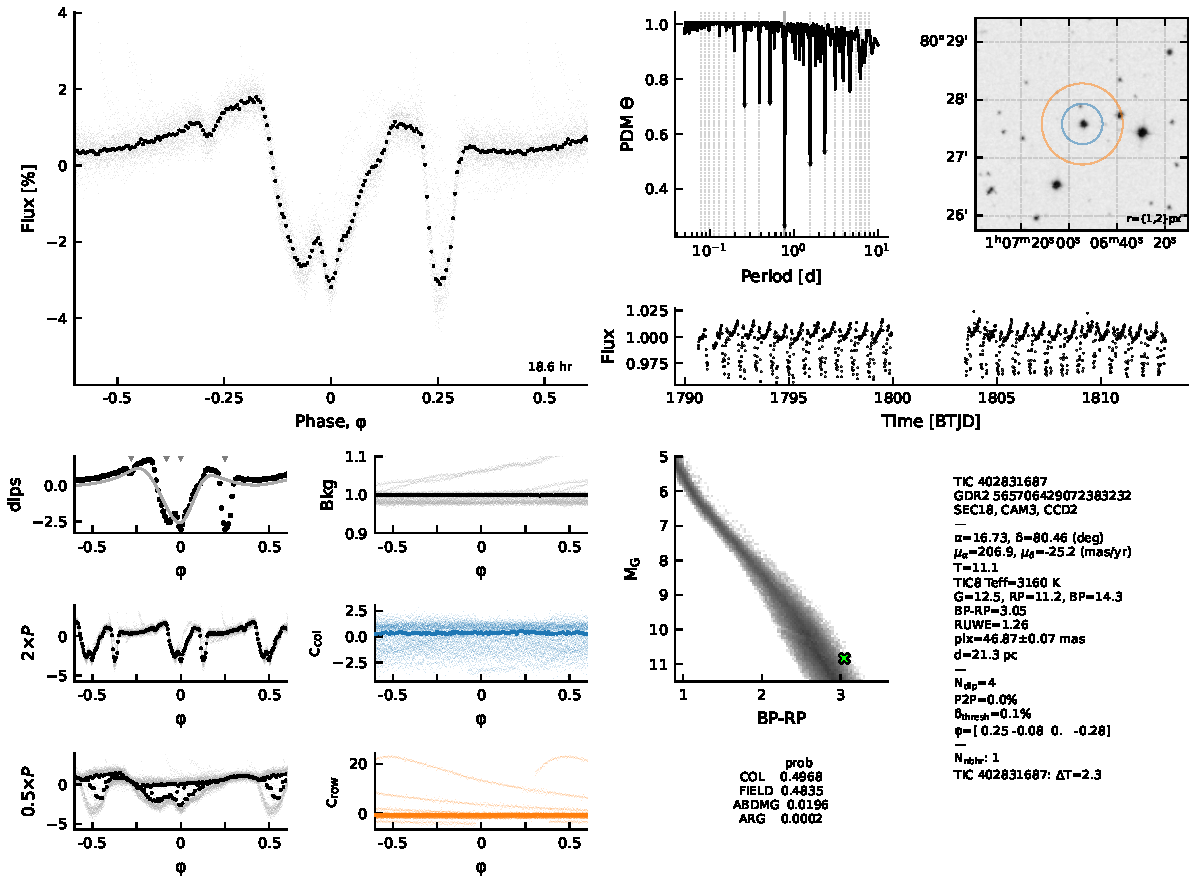
\includegraphics[width=0.96\textwidth]{402980664_S0018_120sec_cpvvetter.pdf}
		\vspace{-0.45cm}
		\caption{
      {\bf Validation plots used to label CQVs}.  The complete figure
      set, with one image per sector for each of \ncpvsfound\ objects
      is available online {\bf For internal collaboration review:
      \url{https://www.dropbox.com/scl/fo/zlj3txot4cvymfb22wewu/h?dl=0&rlkey=3ec5f9o5xewrixzfkhkdenopa}}.
      Panels are as follows.
      {\it a)}: Phase-folded light curve; gray points are raw 2-minute
      data and black points are binned to 200 points per cycle.
      {\it b)}: Phase-dispersion minimization (PDM) periodogram.
      Dotted lines show up to the 10$^{\rm th}$ harmonic and
      subharmonic.
      {\it c)}: DSS finder chart, with 1- and 2-TESS pixel radius
      circles displayed for scale.
      {\it d)}: Cleaned light curve, binned to 20-minute cadence, in
      Barycentric TESS Julian Date (BTJD).
      {\it e)}: Phase-folded light curve, binned to 100 points per
      cycle.  The gray line denotes the automated spline-fit to the
      wrapped phase-folded light curve, and small gray triangles
      denote automatically identified local minima.
      {\it f)}: Phase-folded light curve at twice the peak period.
      {\it g)}: Phase-folded light curve at half the peak period.
      {\it h)}: Phase-folded time-series within the ``background''
      aperture defined in the SPOC light curves.
      {\it i)}: Phase-folded flux-weighted centroid in the column
      direction.
      {\it j)}: Phase-folded flux-weighted centroid in the row
      direction.
      {\it k)}: Gaia DR2 color--absolute magnitude diagram.     
      {\it l)}: Information from Gaia DR2, TIC8, and the automated
      dip-counting search pipeline.  ``Neighbors'', abbreviated
      ``nbhr'', are listed within apparent distances of 2 TESS pixels
      if $\Delta T$$<$2.5.
      {\it m)}: BANYAN-$\Sigma$ v1.2 association probabilities, calculated
      using positions, proper motions, and the parallax.
      }
		\label{fig:vet}
	\end{center}
\end{figure*}


\section{LP 12-502}
\label{app:lp}

{\it The light curve}---
Figure~\ref{fig:lp2} shows another alternative view of
Figure~\ref{fig:lp}, but arranged to enable easy visual appreciation
of transit timing changes, rather than transit depth changes.  A
best-fitting two-harmonic sinusoid has been independently fitted and
subtracted from the Sector 18-19 data, 25-26 data, and 53, 58, and 59
data.

Finally, Figure~\ref{fig:lpriver0} shows ``river plots'' of the
same data, split into very similar intervals:
the Sector 18-19 data, 25-26 data, 53 data, and 58-59 data.
State changes are evident in these plots whenever there is a sudden
change in color.
{\bf todo: fix missing data to be different from the flare color} 


\begin{figure*}[!t]
	\begin{center}
    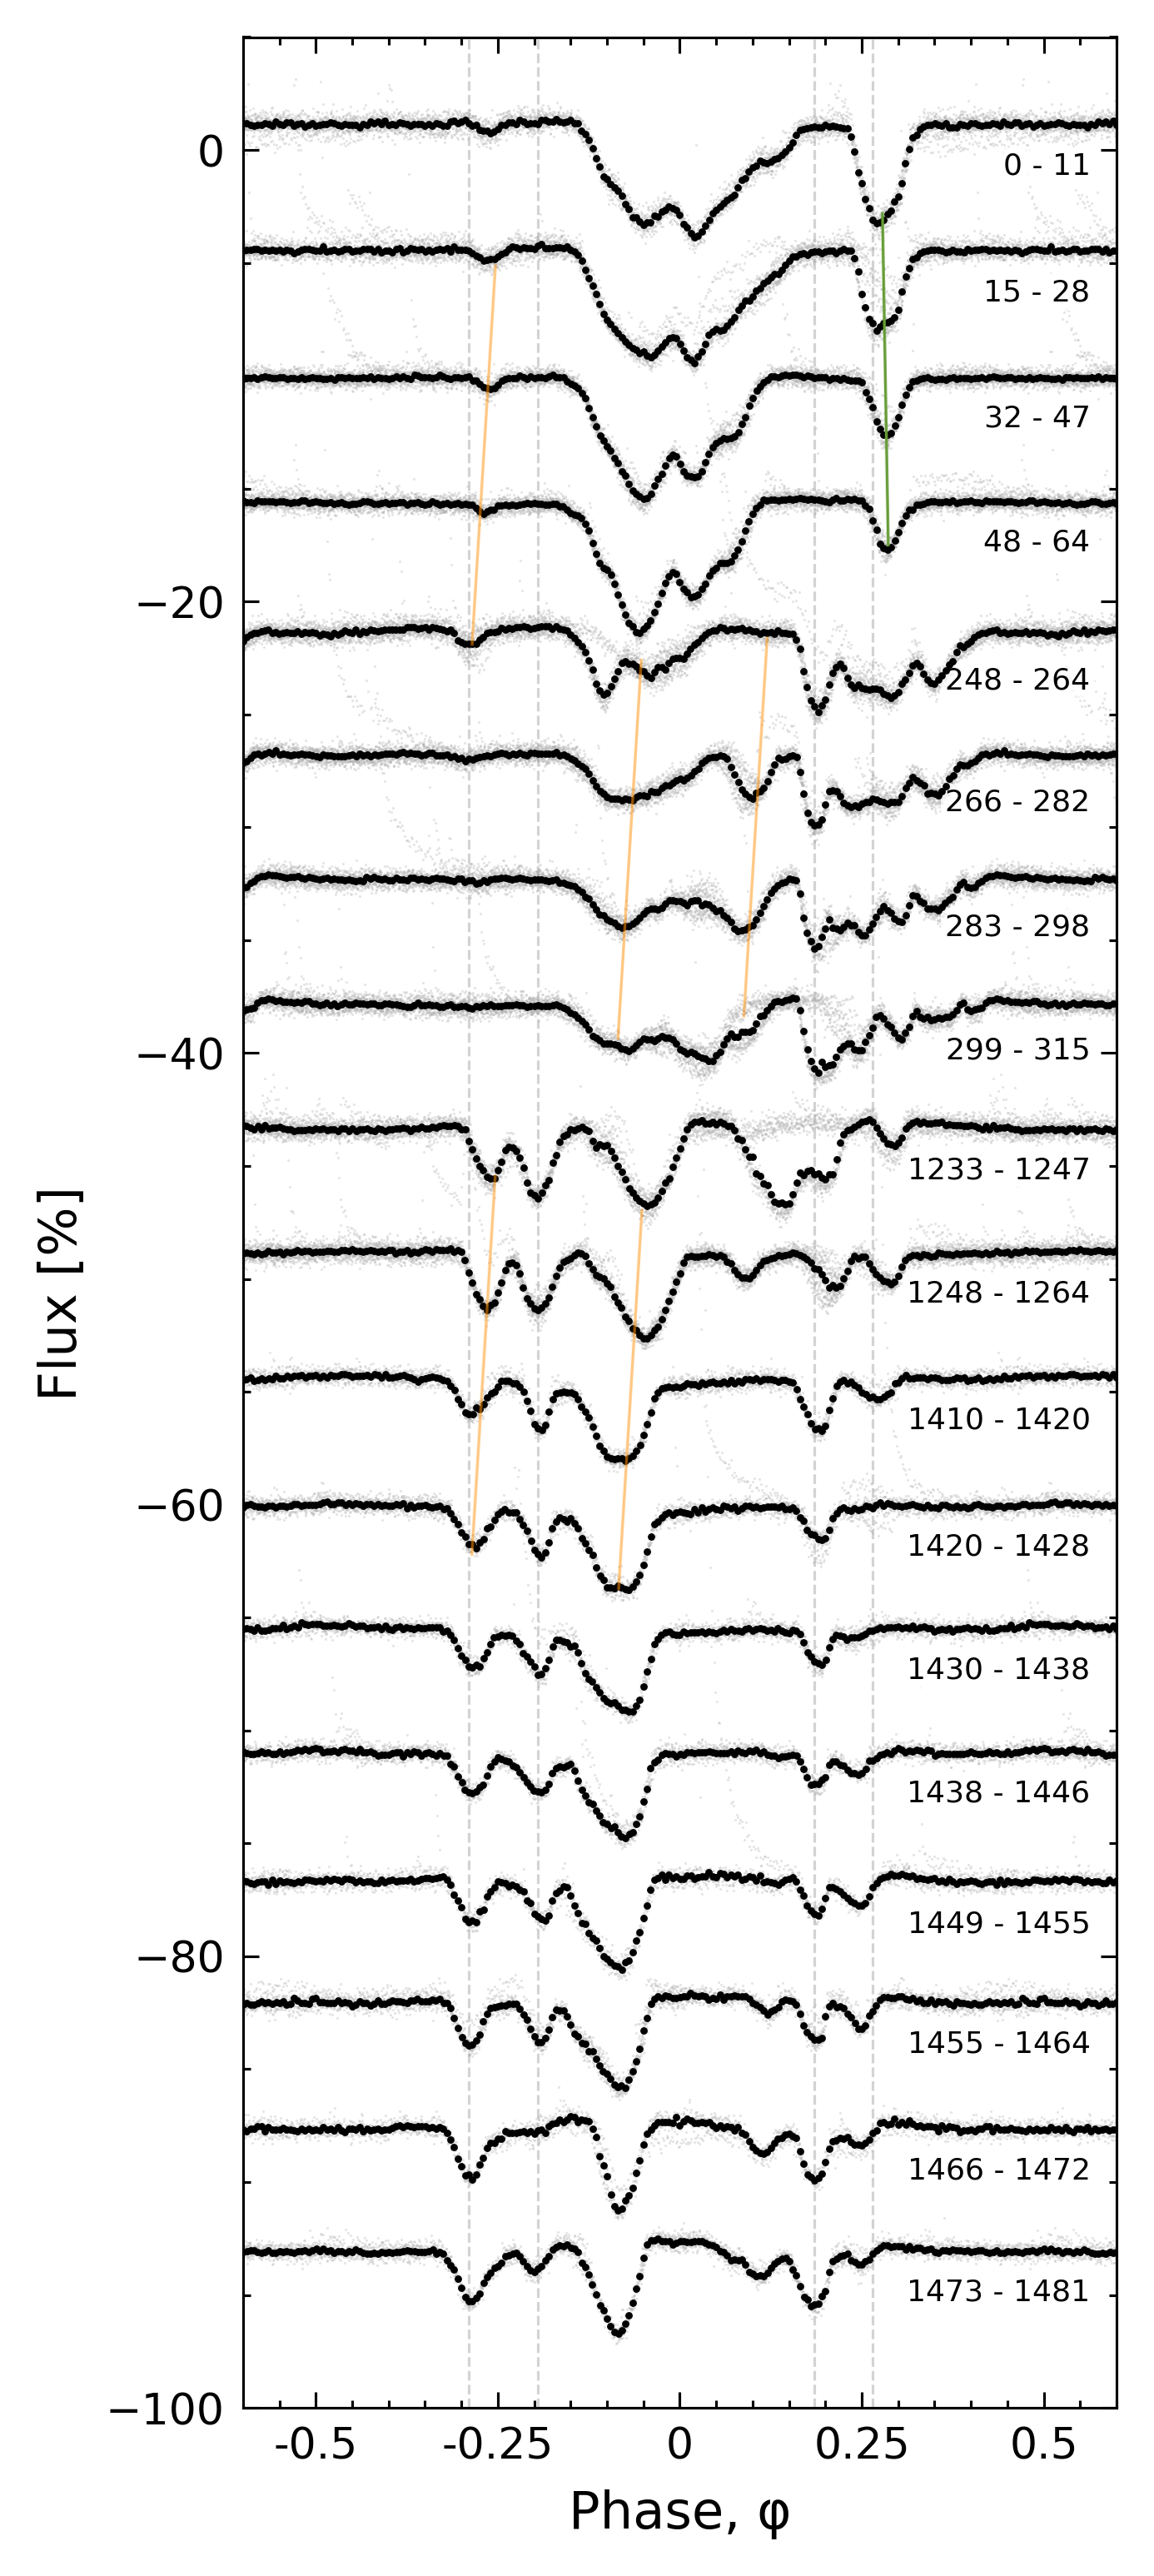
\includegraphics[width=0.45\textwidth]{ANNOTATED_resid_TIC_402980664_P18.5611_2min_phase_timegroups.png}
    	\end{center}
    \vspace{-0.4cm}
		\caption{
	      {\bf Alternative view of the evolution of LP 12-502}
	      (Figure~\ref{fig:lp}), arranged to emphasize changes in transit
	      times.  There are 200 binned black points per cycle; a two-harmonic
	      sinusoid has been subtracted over specific chunks in time ({\bf see text}).
	      Vertical gray lines are underplotted to help guide the eye to instances
	      in which preferred dip phases synchronize over long baselines.
	      The orange and green lines guide the eye to where dips
	      appear to change the positions of their local minima.
		}
		\label{fig:lp2}
\end{figure*}


\begin{figure*}[!t]
	\begin{center}
		\subfloat{
			\includegraphics[width=0.43\textwidth]{TIC402980664_river_gist_stern_0_64_manual_20230617_mask_v0_nterms2_vmin-0.04000_vmax0.01000.png}
			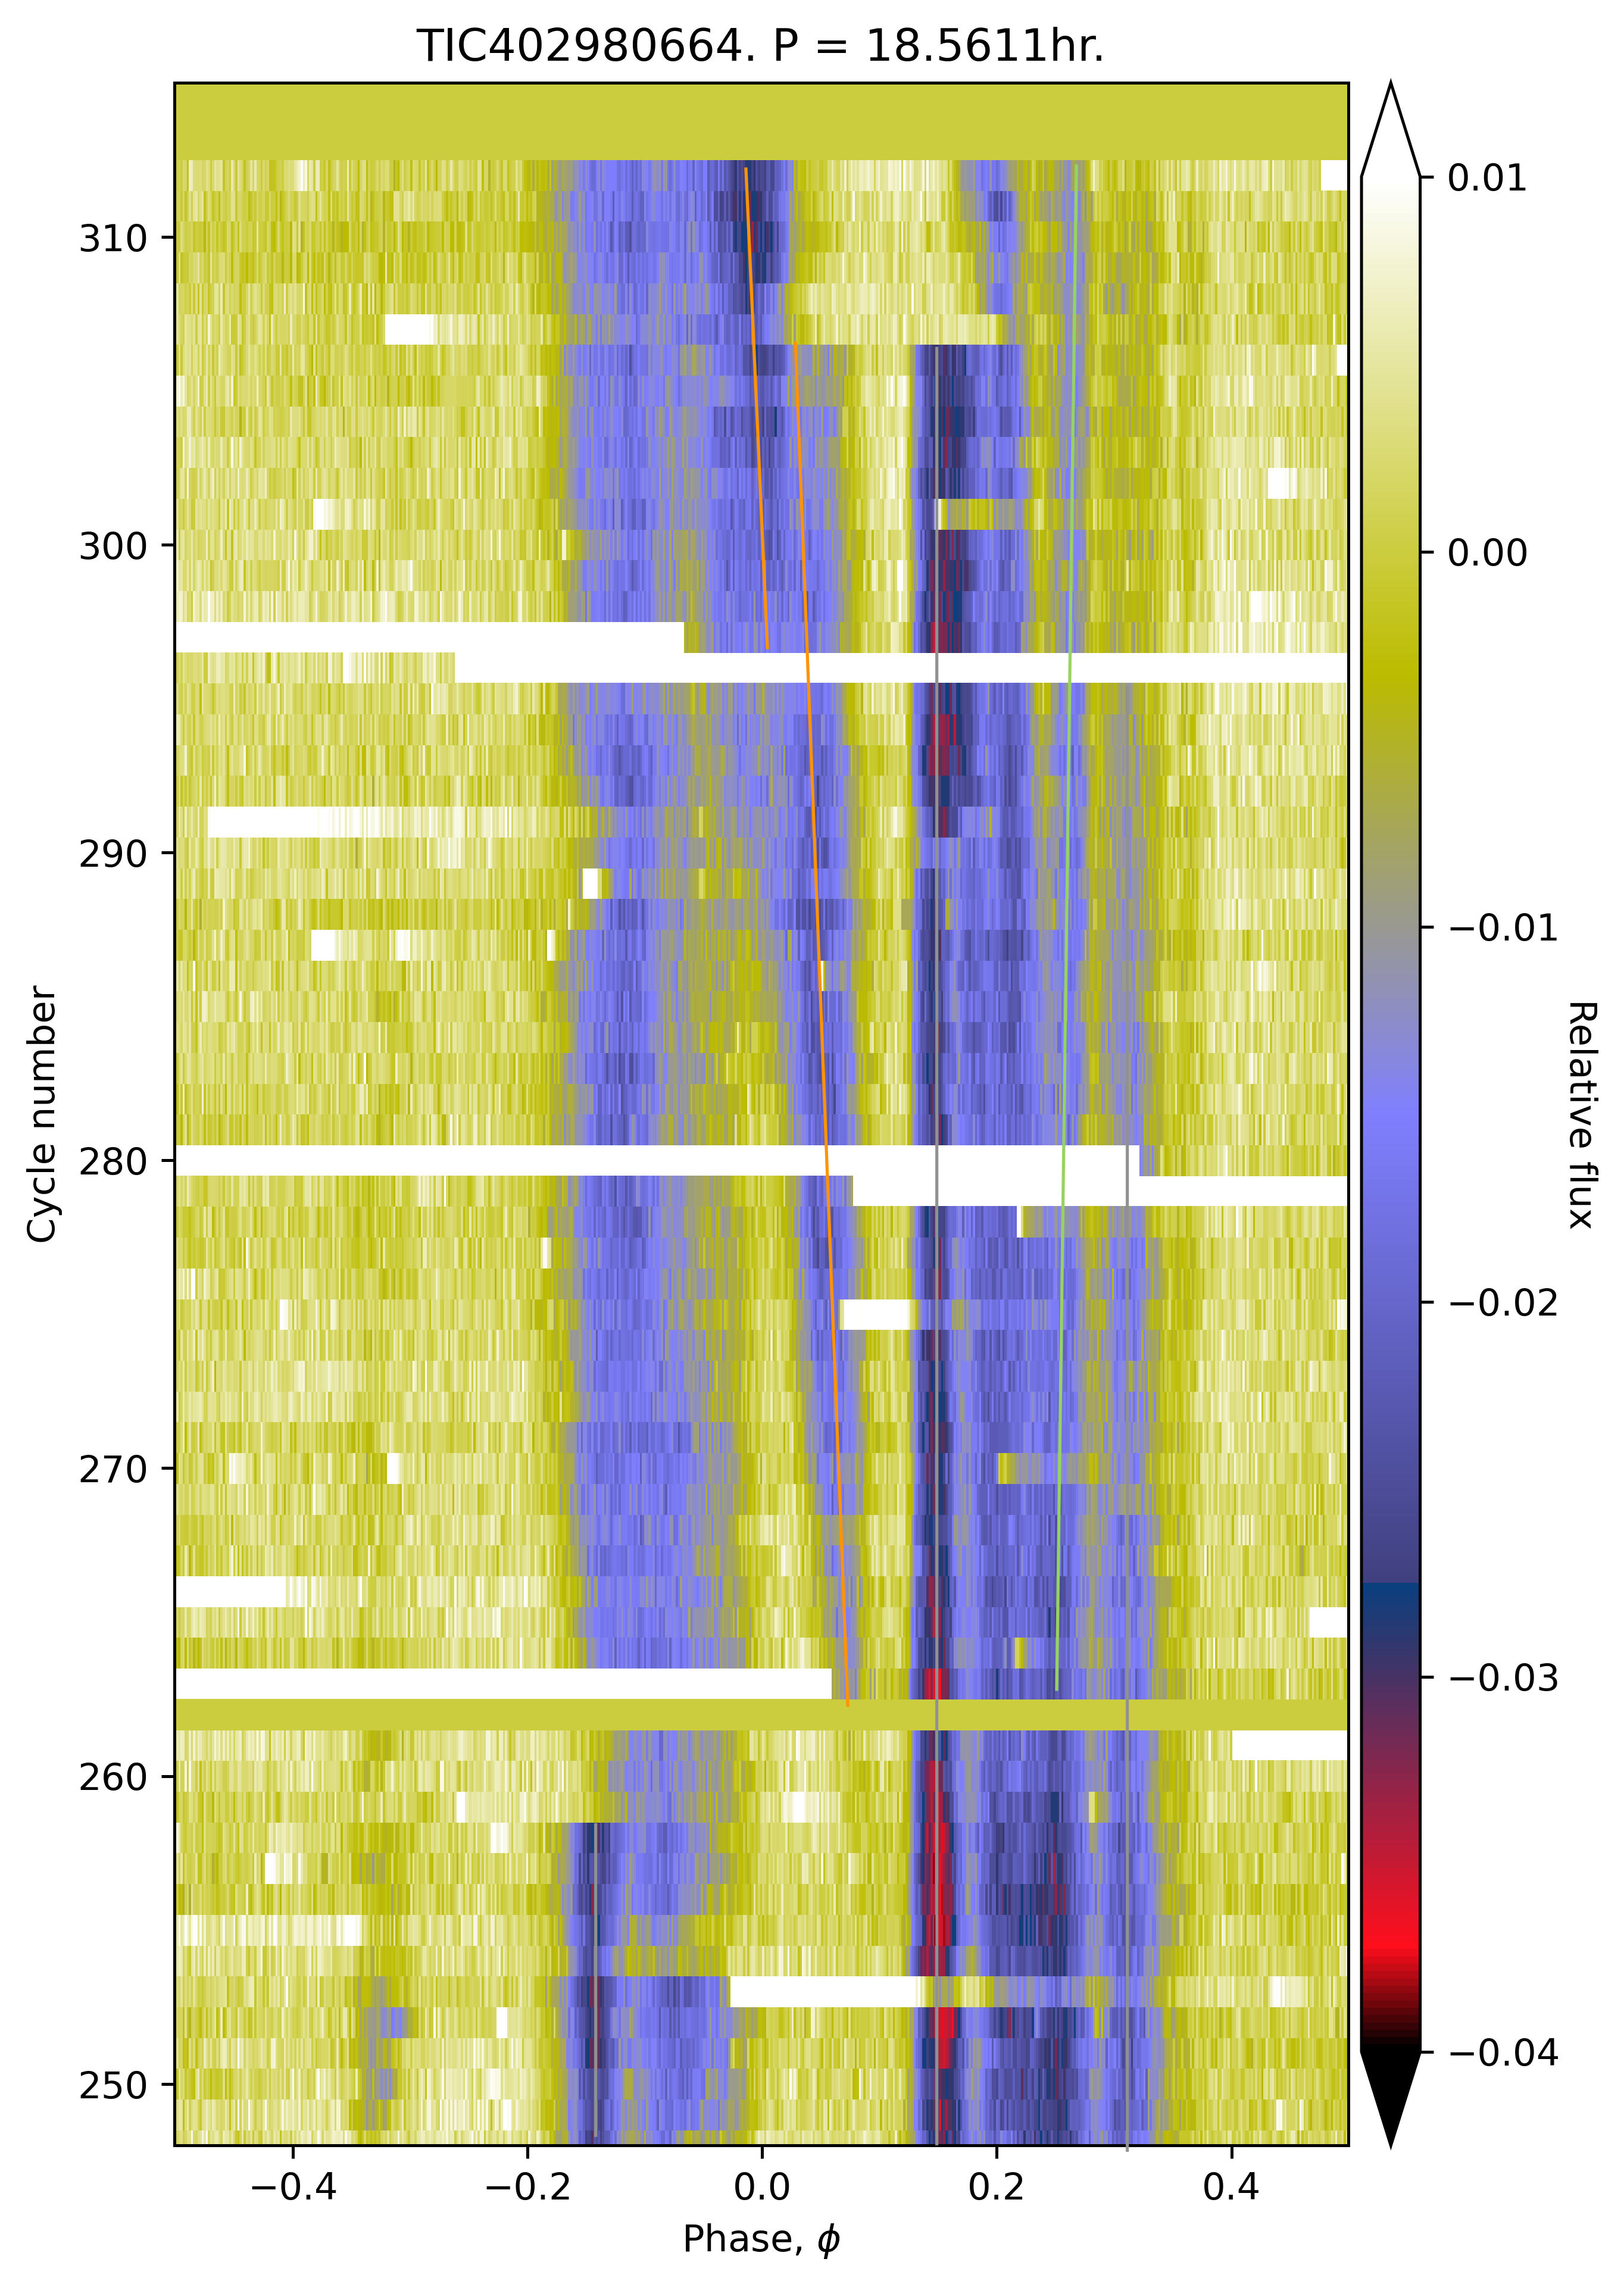
\includegraphics[width=0.43\textwidth]{ANNOTATED_TIC402980664_river_gist_stern_248_315_manual_20230617_mask_v0_nterms2_vmin-0.04000_vmax0.01000.png}
		}
	\vspace{-1cm}
			\subfloat{
		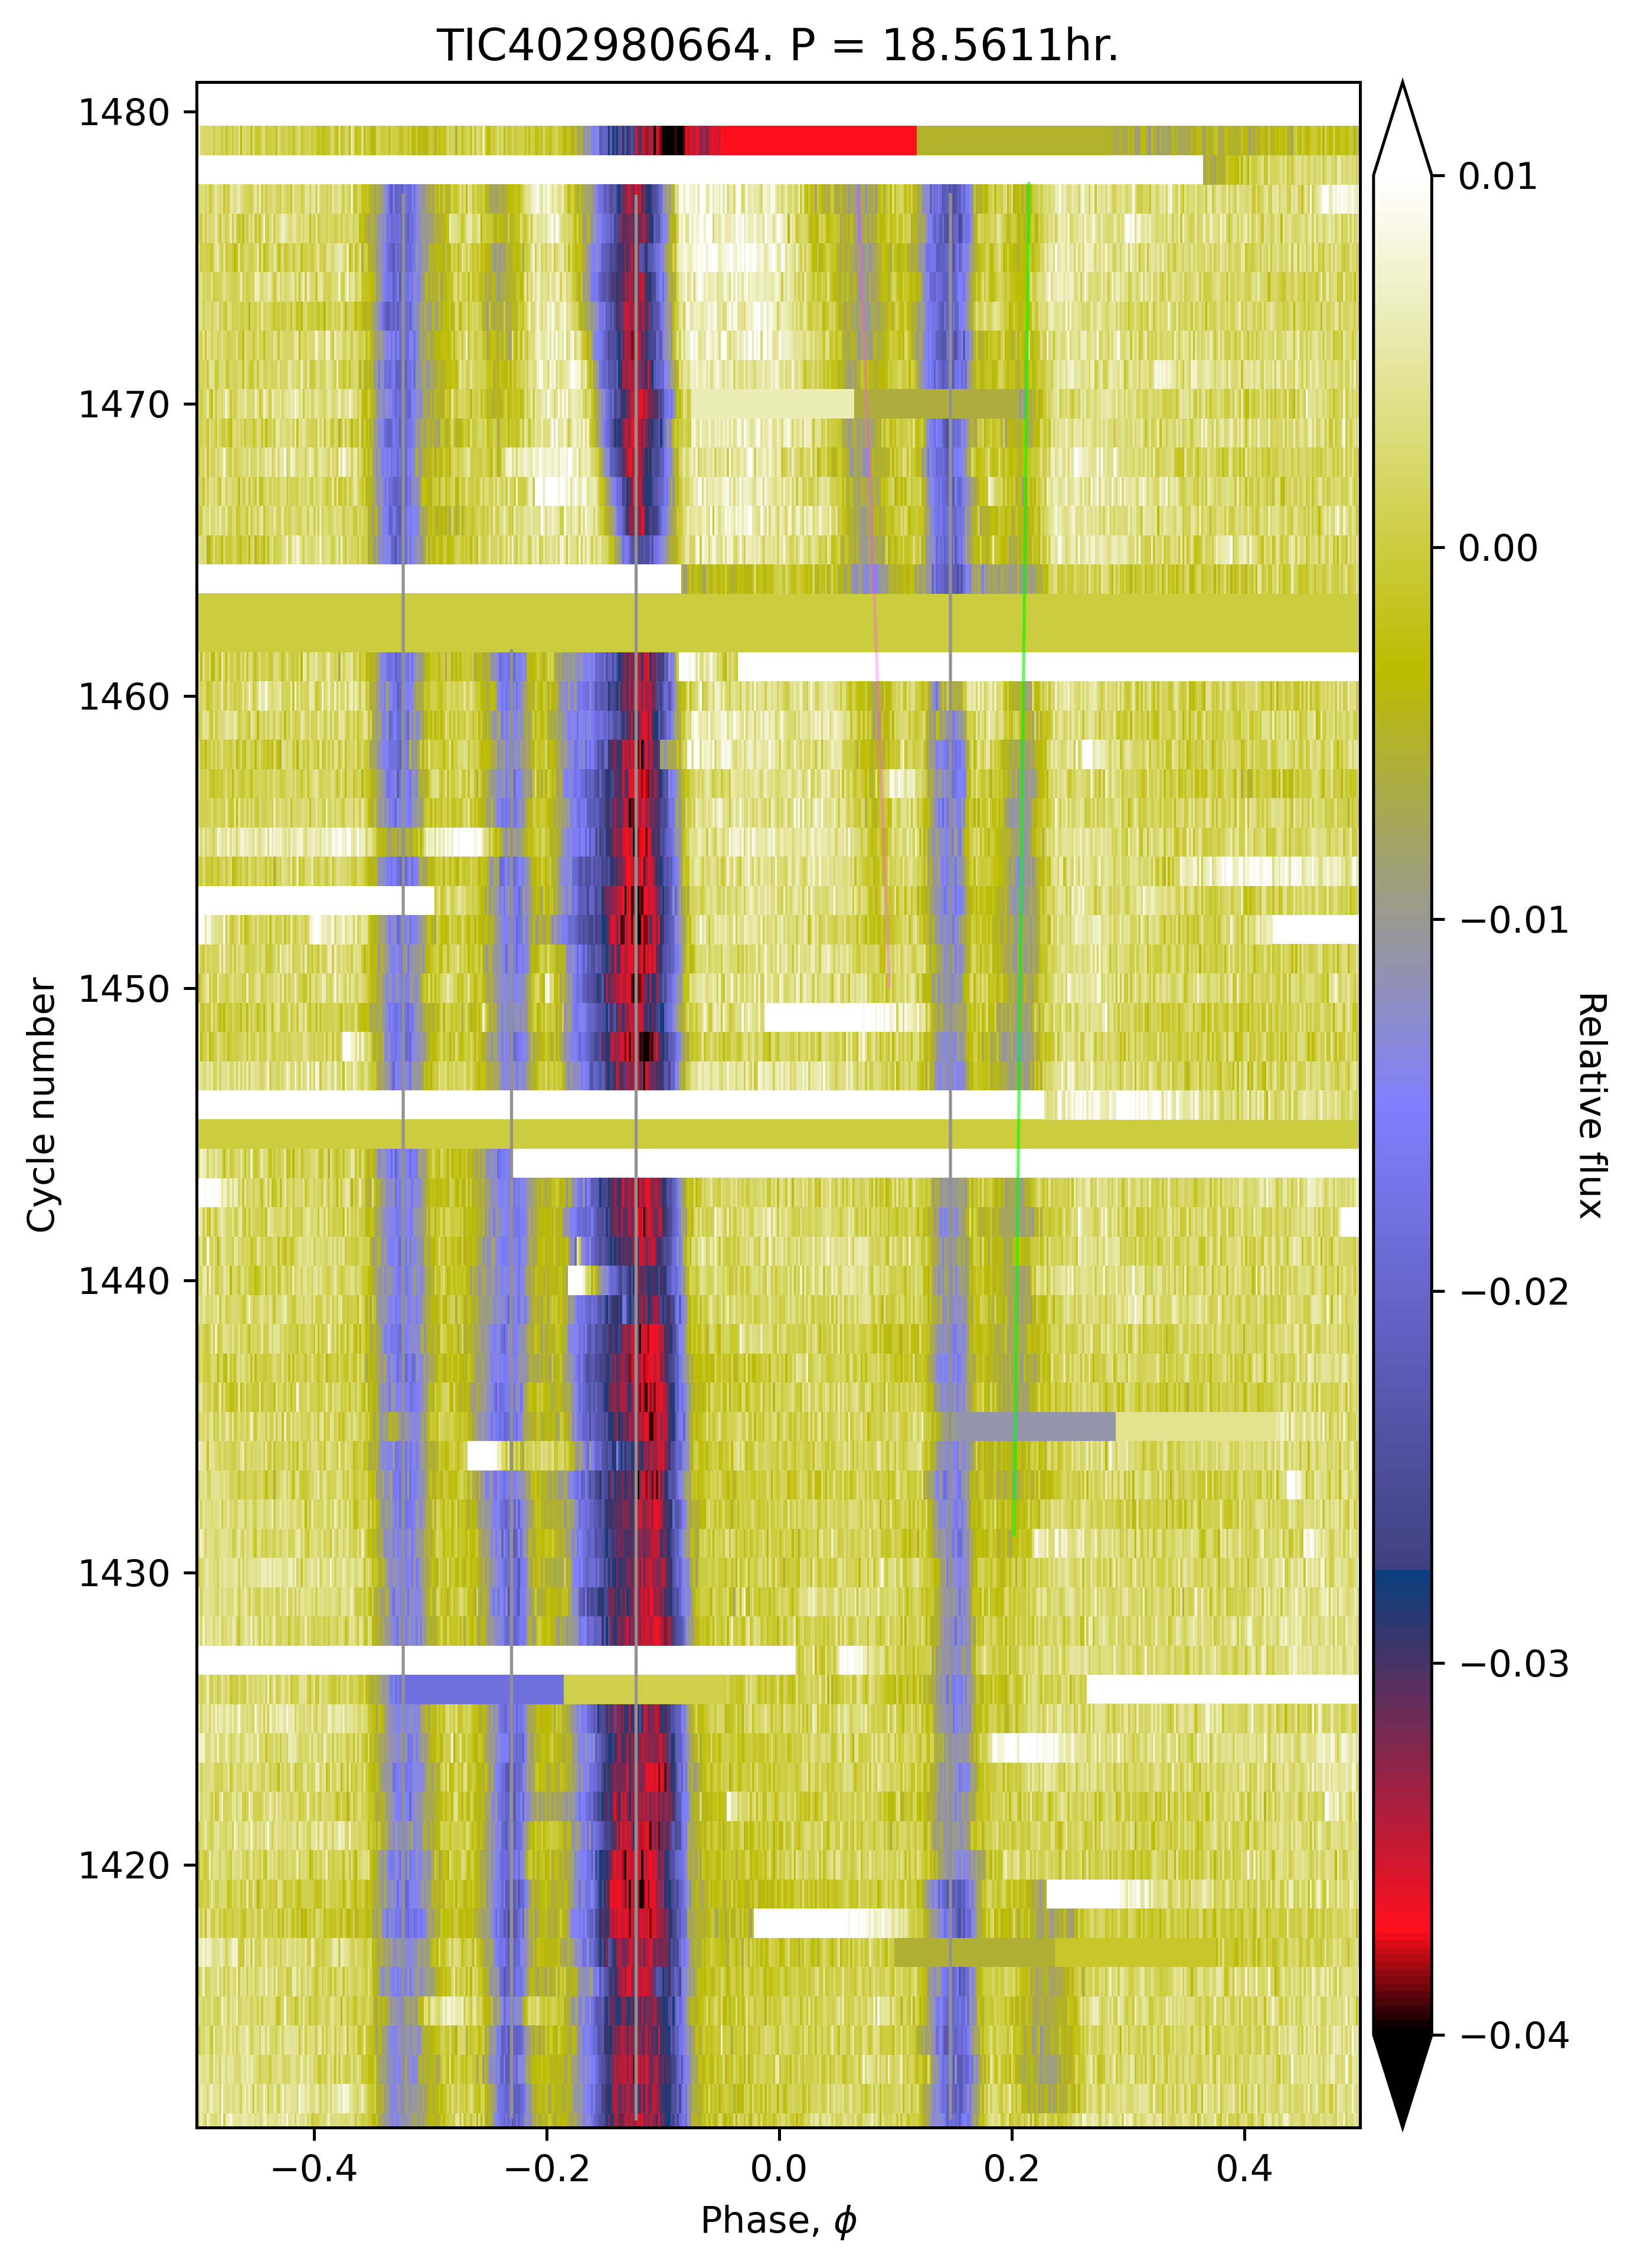
\includegraphics[width=0.43\textwidth]{ANNOTATED_TIC402980664_river_gist_stern_1411_1481_manual_20230617_mask_v0_nterms2_vmin-0.04000_vmax0.01000.png}
				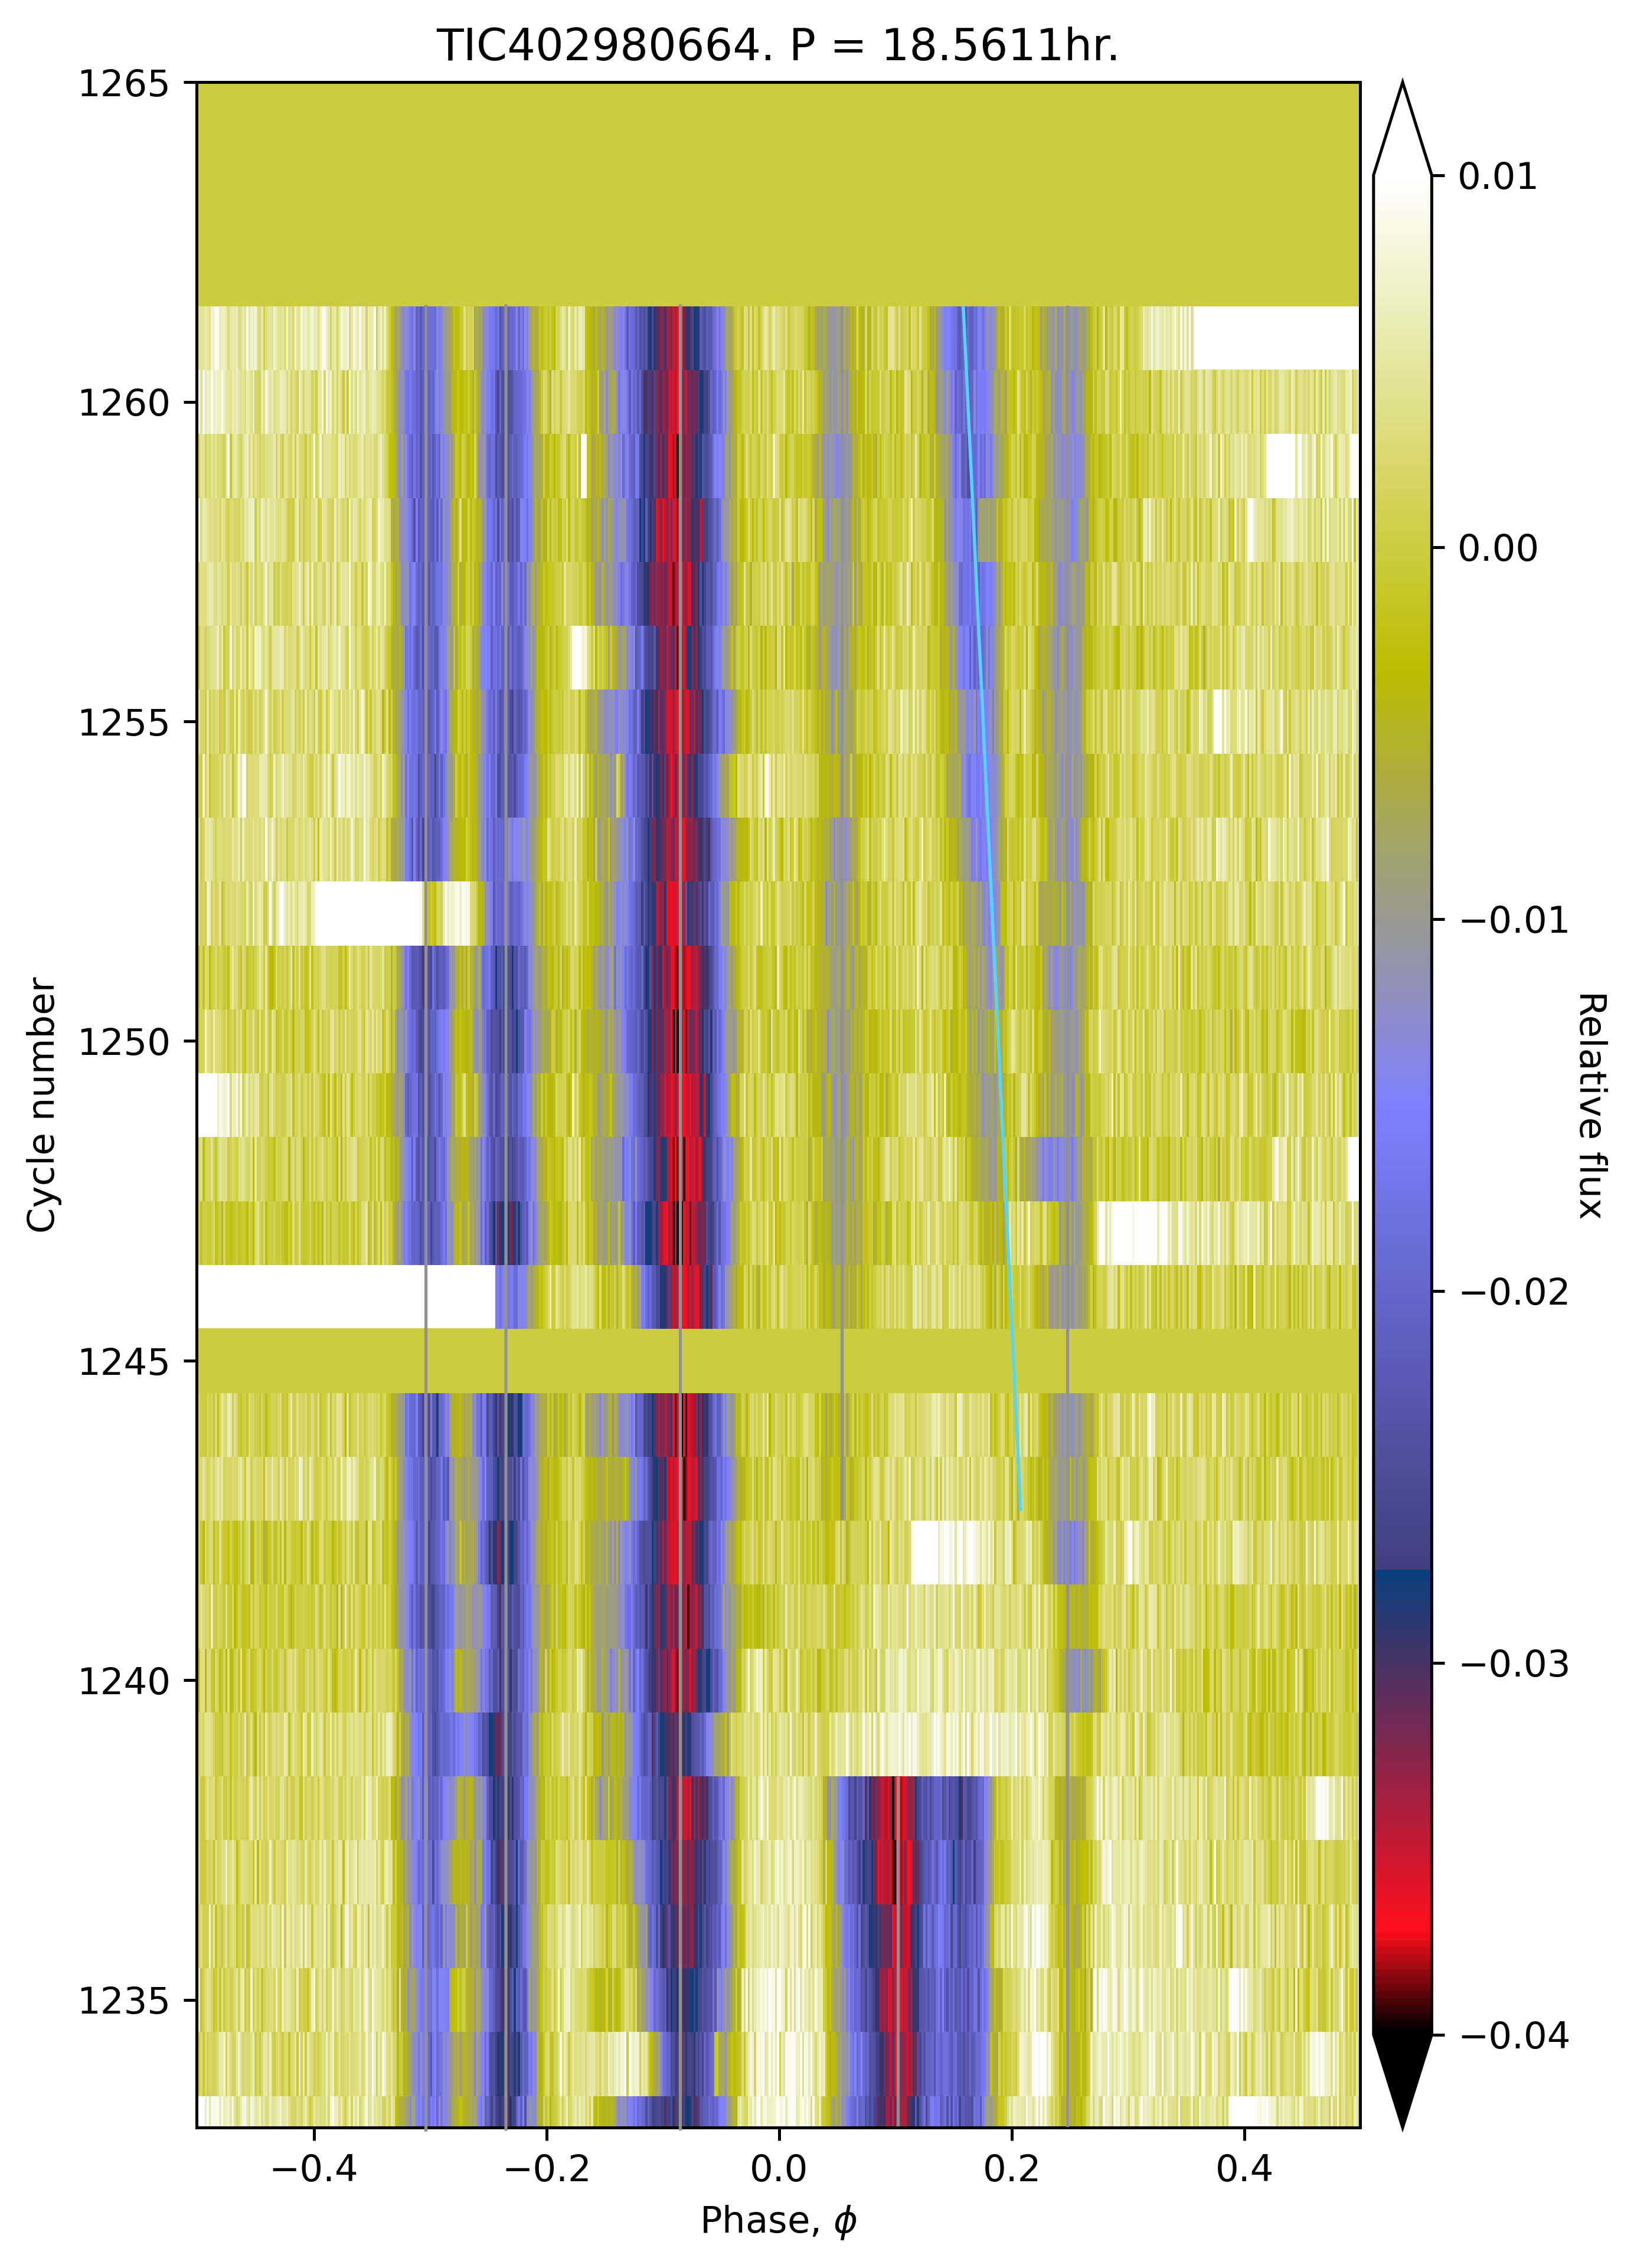
\includegraphics[width=0.43\textwidth]{ANNOTATED_TIC402980664_river_gist_stern_1233_1265_manual_20230617_mask_v0_nterms2_vmin-0.04000_vmax0.01000.png}
	}
	\end{center}
	\vspace{-0.4cm}
	\caption{
    {\bf River plots of LP 12-502}, showing (clockwise from top-left)
    Sectors 18-19, 25-26, 53, and 58-59.  A two-harmonic sinusoid has
    been subtracted over specific chunks in time ({\bf see text}).
    For Sectors 25-26 (cycles 248-315), three periods are overplotted:
    $P$=18.5611\,hr (gray vertical line); 18.5404\,hr (orange); 18.5683\,hr (green).
    For Sector 53, gray is identical, while cyan is 18.5145\,hr.
    For Sectors 58-59, the magenta line is 18.5473\,hr, and the green
    line is 18.5672\,hr.
	}
	\label{fig:lpriver0}
\end{figure*}


\section{No additional power at 20~second cadence}

Going from K2 to TESS, an important discovery was that the CQV shapes
can significantly evolve, since the stars can vary over timescales of just a few minutes.
We observed a set of CQVs between 2020 and 2021 using the TESS 20-second
cadence mode (TESS DDT029).
{\bf todo: list the stars.  todo: examine the 2min vs 20sec periodograms, and summarize in a few
sentences whether any difference is there.}



\section{Chromaticity in TIC 262400835}

TIC~262400835 ($d$=174\,pc) is formally outside the scope of the
current work.  However, this CQV was observed using MuSCAT2 on 2020
December 12, 13, and 16, and the results are pertinent enough to the
present work.
{\bf todo: describe observations}.

We include {\bf a table of the photometry} here to enable potential
future deeper analyses of the chromaticity of this object class.

Generally, these data serve as a minor addition beyond the
observations that have been acquired by
\citet[e.g.][]{2017PASJ...69L...2O,2020PASJ...72...23T,2022AJ....163..144G,2023MNRAS.518.2921K}
on this topic.  \citet{2023MNRAS.518.2921K} provides what we find to
be the most lucid summary, and we quote: ``amplitudes are almost
always larger, the shorter the wavelength of the filter, but the
relationship can be weak or non-monotonic.''

\begin{figure*}[!t]
	\begin{center}
    \includegraphics[width=0.45\textwidth]{TIC262400835_multicolor_phase_stacked.pdf}
    	\end{center}
    \vspace{-0.4cm}
		\caption{
	      {\bf Chromaticity in TIC~262400835}.
		}
		\label{fig:muscat}
\end{figure*}



\clearpage
\listofchanges


\end{document}
